%to do: slide 15, reduce number of variables
% slide 10, seperate a_t and b_t figures, give a_t first



%\documentclass[12pt,reqno,utf8,utf8x]{article}

\documentclass[8pt,aspectratio=169]{beamer}
\usepackage{natbib}
\usepackage{tikz}
%\usetheme[progressbar=frametitle]{metropolis}
\usepackage[utf8]{inputenc}
\usepackage{graphicx}
\usepackage{animate}
\graphicspath{ {images/} }
\usepackage{geometry}
\usepackage{subfigure}
\usepackage[english]{babel}
\usepackage[]{xcolor}

\usepackage{amsmath,amsfonts,amssymb}
\usepackage{verbatim}
\usepackage{gensymb}
\usepackage{bm}
\usepackage{float}
\usepackage{rotating}
\usepackage{graphicx}
\usepackage{setspace}
\numberwithin{equation}{section}
\usepackage{fancyhdr}
\usepackage{color}

%\usetheme{Singapore}
\usecolortheme{Lily}
\title{\bf Update on the Sectoral DSGE Model}
	
\definecolor{Gray}{gray}{0.9}
\definecolor{LightCyan}{rgb}{0.88,1,1}

\author{Marc Hinterschweiger, Kunal Khairnar, Tolga Ozden, Tom Stratton}

%\AtBeginSubsection[]
%{
%  \begin{frame}<beamer>{Outline}
%    \tableofcontents[]
%  \end{frame}
%}

\begin{document}
\titlepage
\begin{frame}{Overview}




\begin{itemize}

\item Model overview
\vspace{5 mm}
\item Estimation highlights
\vspace{5 mm}
\item Policy analysis \& Counterfactuals
\vspace{5 mm}
\item Interest rate pass-through \& Prudential policy

\end{itemize}


\end{frame}


\begin{frame}{Model Overview}

\begin{figure}
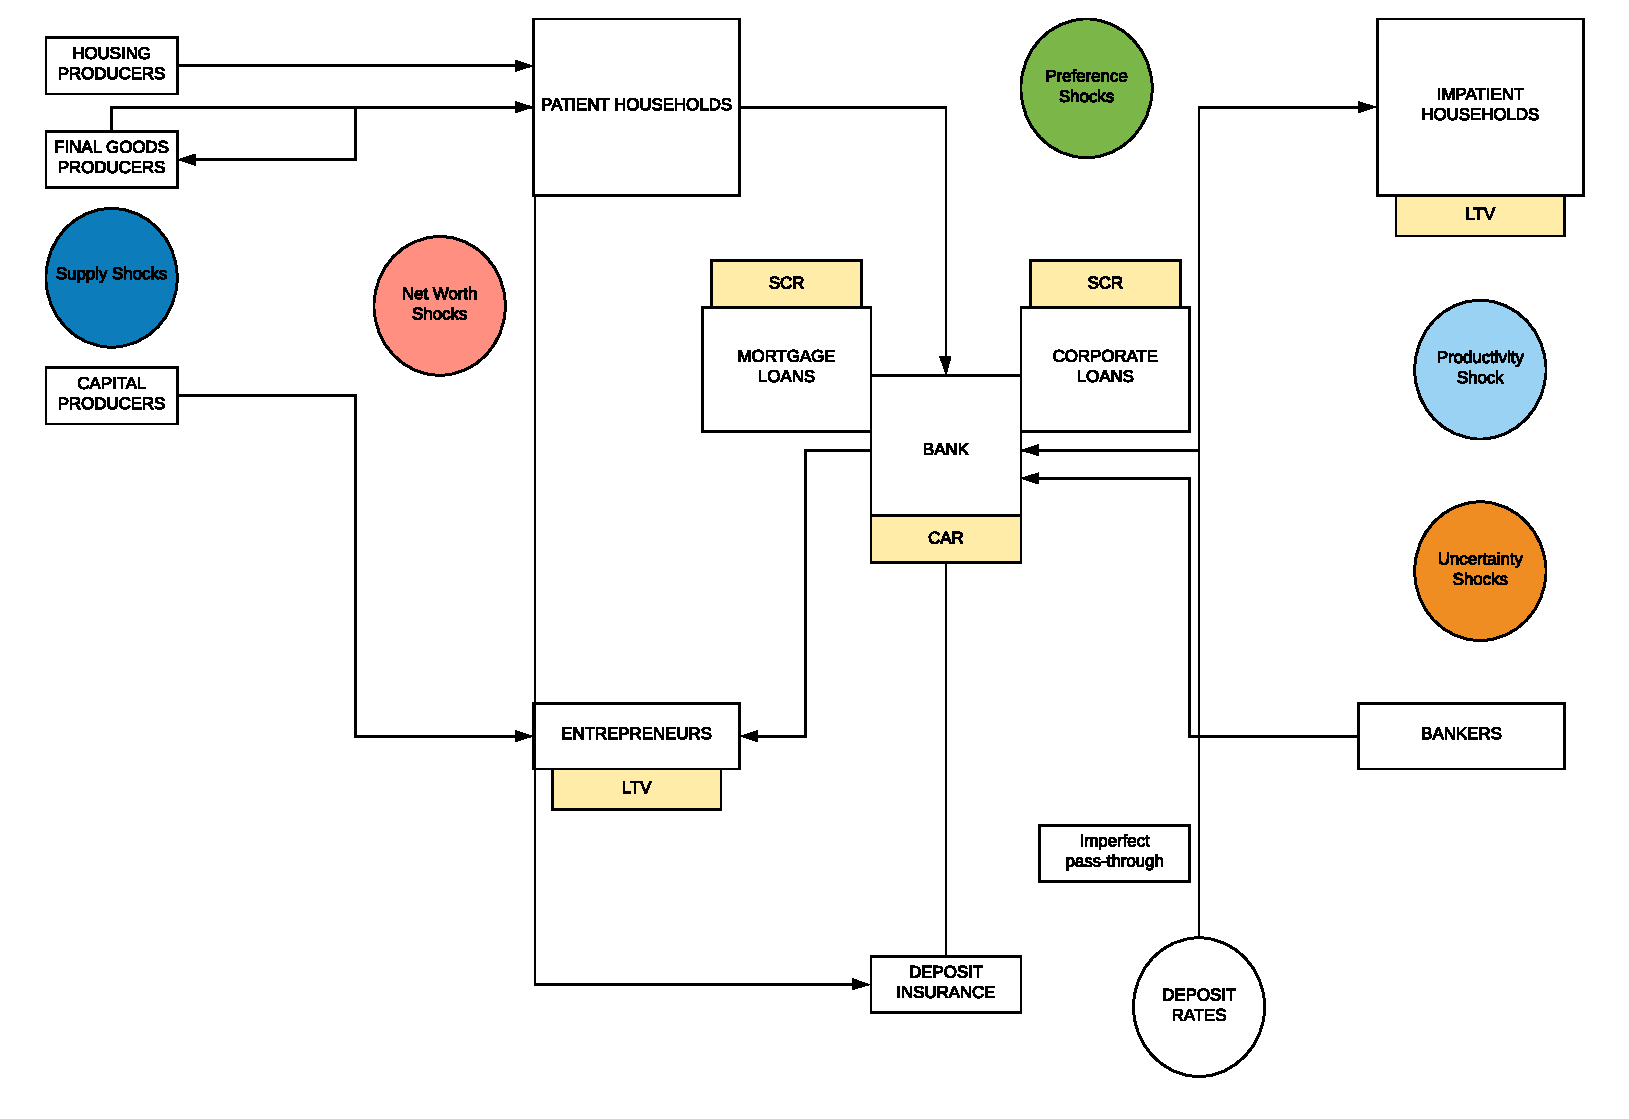
\includegraphics[scale=0.45]{3d_model_overview.pdf}
\end{figure}

\end{frame}



\begin{frame}{Estimation-I}


\begin{itemize}

\item Quarterly data for the U.K. economy over 1998Q1-2016Q4. 
\vspace{5 mm}
\item 10 observables in: 
\vspace{5 mm}
\begin{itemize}
\item Interest rates (Official bank rate, mortgage \& corporate rates)
\vspace{3 mm}
\item Growth rates (Real output, investment, consumption and wages)
\vspace{3 mm}
\item Credit growth rates (Mortgage \& corporate) 
\vspace{3 mm}
\item House price growth
\end{itemize}

\end{itemize}



\end{frame}


\begin{frame}{Estimation-II}

\begin{itemize}

\item Model: $X_t = f(E_tX_{t+1},X_{t-1},\epsilon_t) $
\vspace{5 mm}
\item Linear approximation around steady-state: $X_t = T X_{t-1} + R \epsilon_t $
\vspace{5 mm}
\item Problem: steady-state is not available in closed-form:  has to be numerically approximated for each parameter draw. 
\vspace{5 mm}
\item Solution: the vast majority of parameters affecting the steady-state are calibrated / fixed using conventional values. 
\vspace{5 mm}
\item Prudential regulation parameters fixed at their historical averages. 
\item The remaining parameters estimated using a Bayesian likelihood approach. 

\end{itemize}




\end{frame}


\begin{frame}{Historical Variance Decompositions: Output   Growth }

\begin{itemize}

\item Each variable over the sample is a combination of shocks
\end{itemize}

\begin{figure}
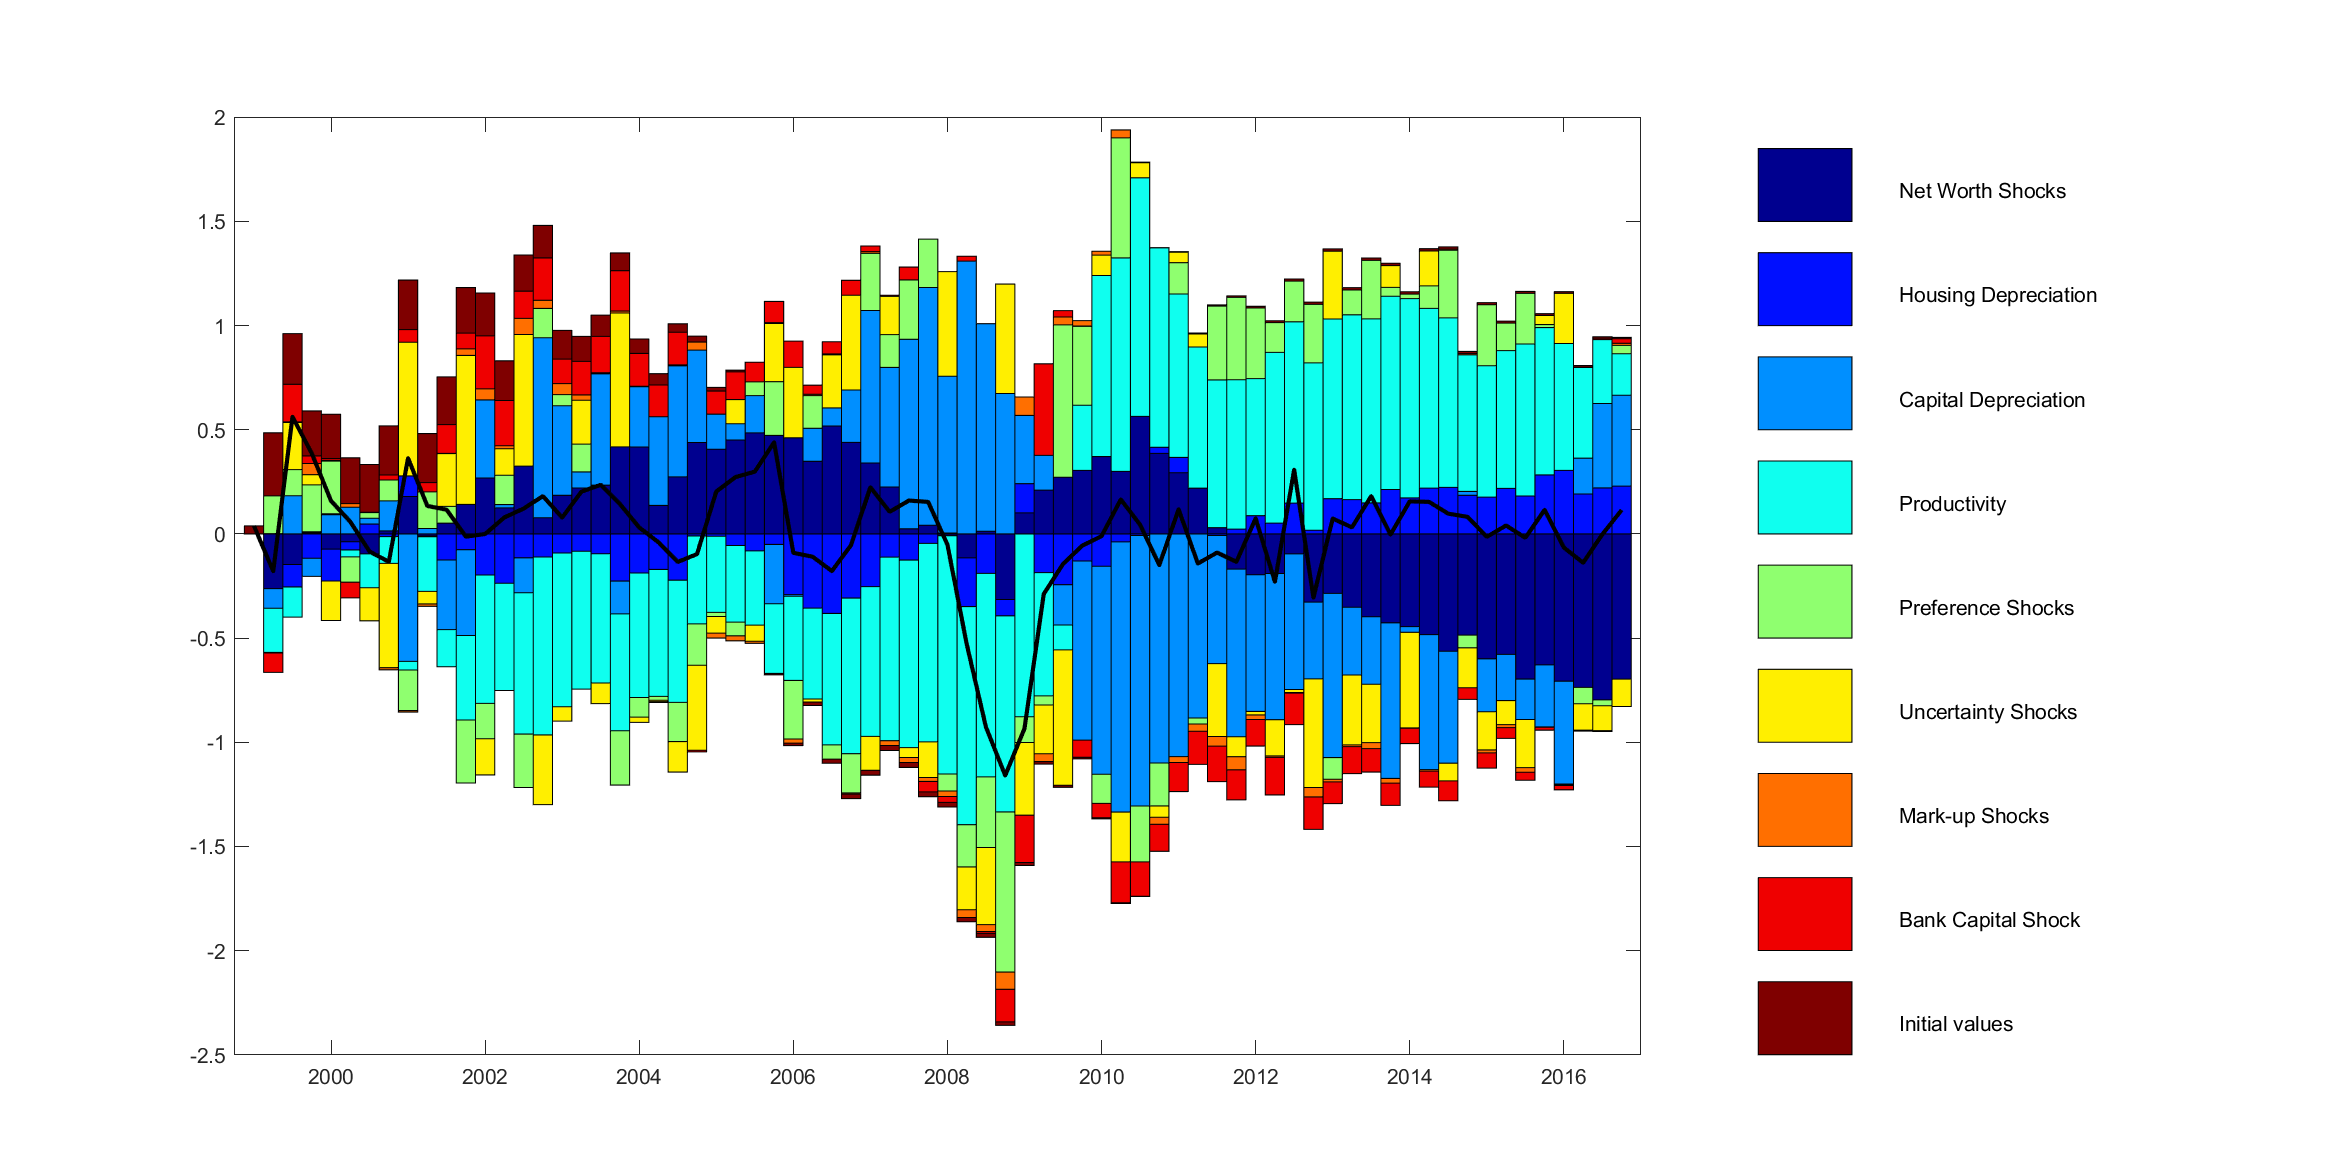
\includegraphics[scale=0.36]{decomp_dy.pdf}
\end{figure}


\end{frame}



\begin{frame}{Historical Variance Decompositions: Consumption Growth }

\begin{itemize}

\item Each variable over the sample is a combination of shocks
\end{itemize}

\begin{figure}
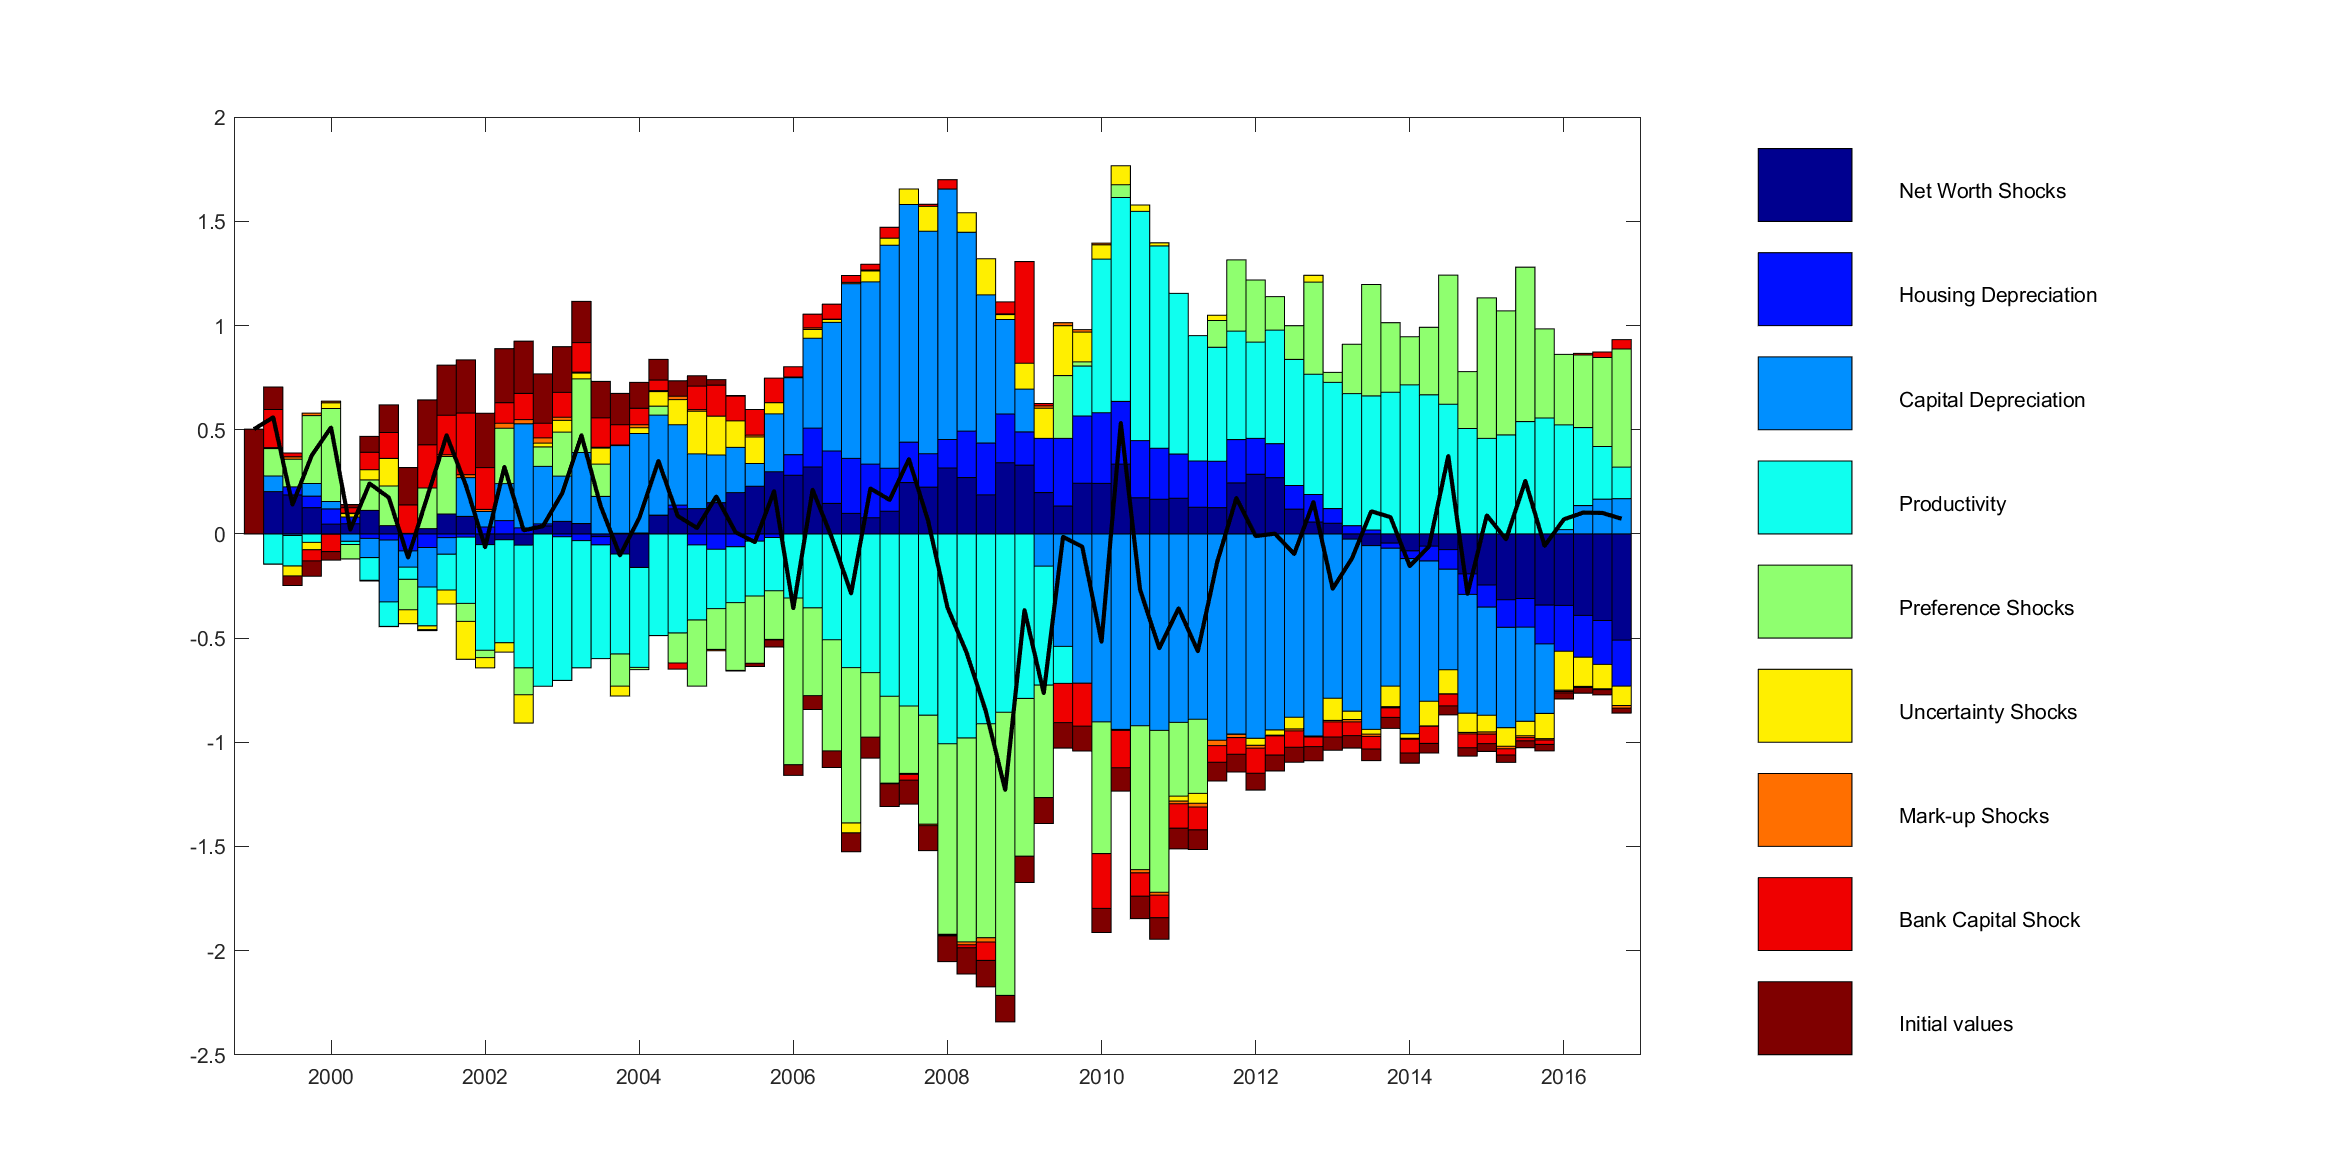
\includegraphics[scale=0.36]{decomp_dc.pdf}
\end{figure}


\end{frame}


\begin{frame}{Historical Variance Decomposition: Household Lending Growth }
\begin{itemize}

\item Each variable over the sample is a combination of shocks
\end{itemize}

\begin{figure}
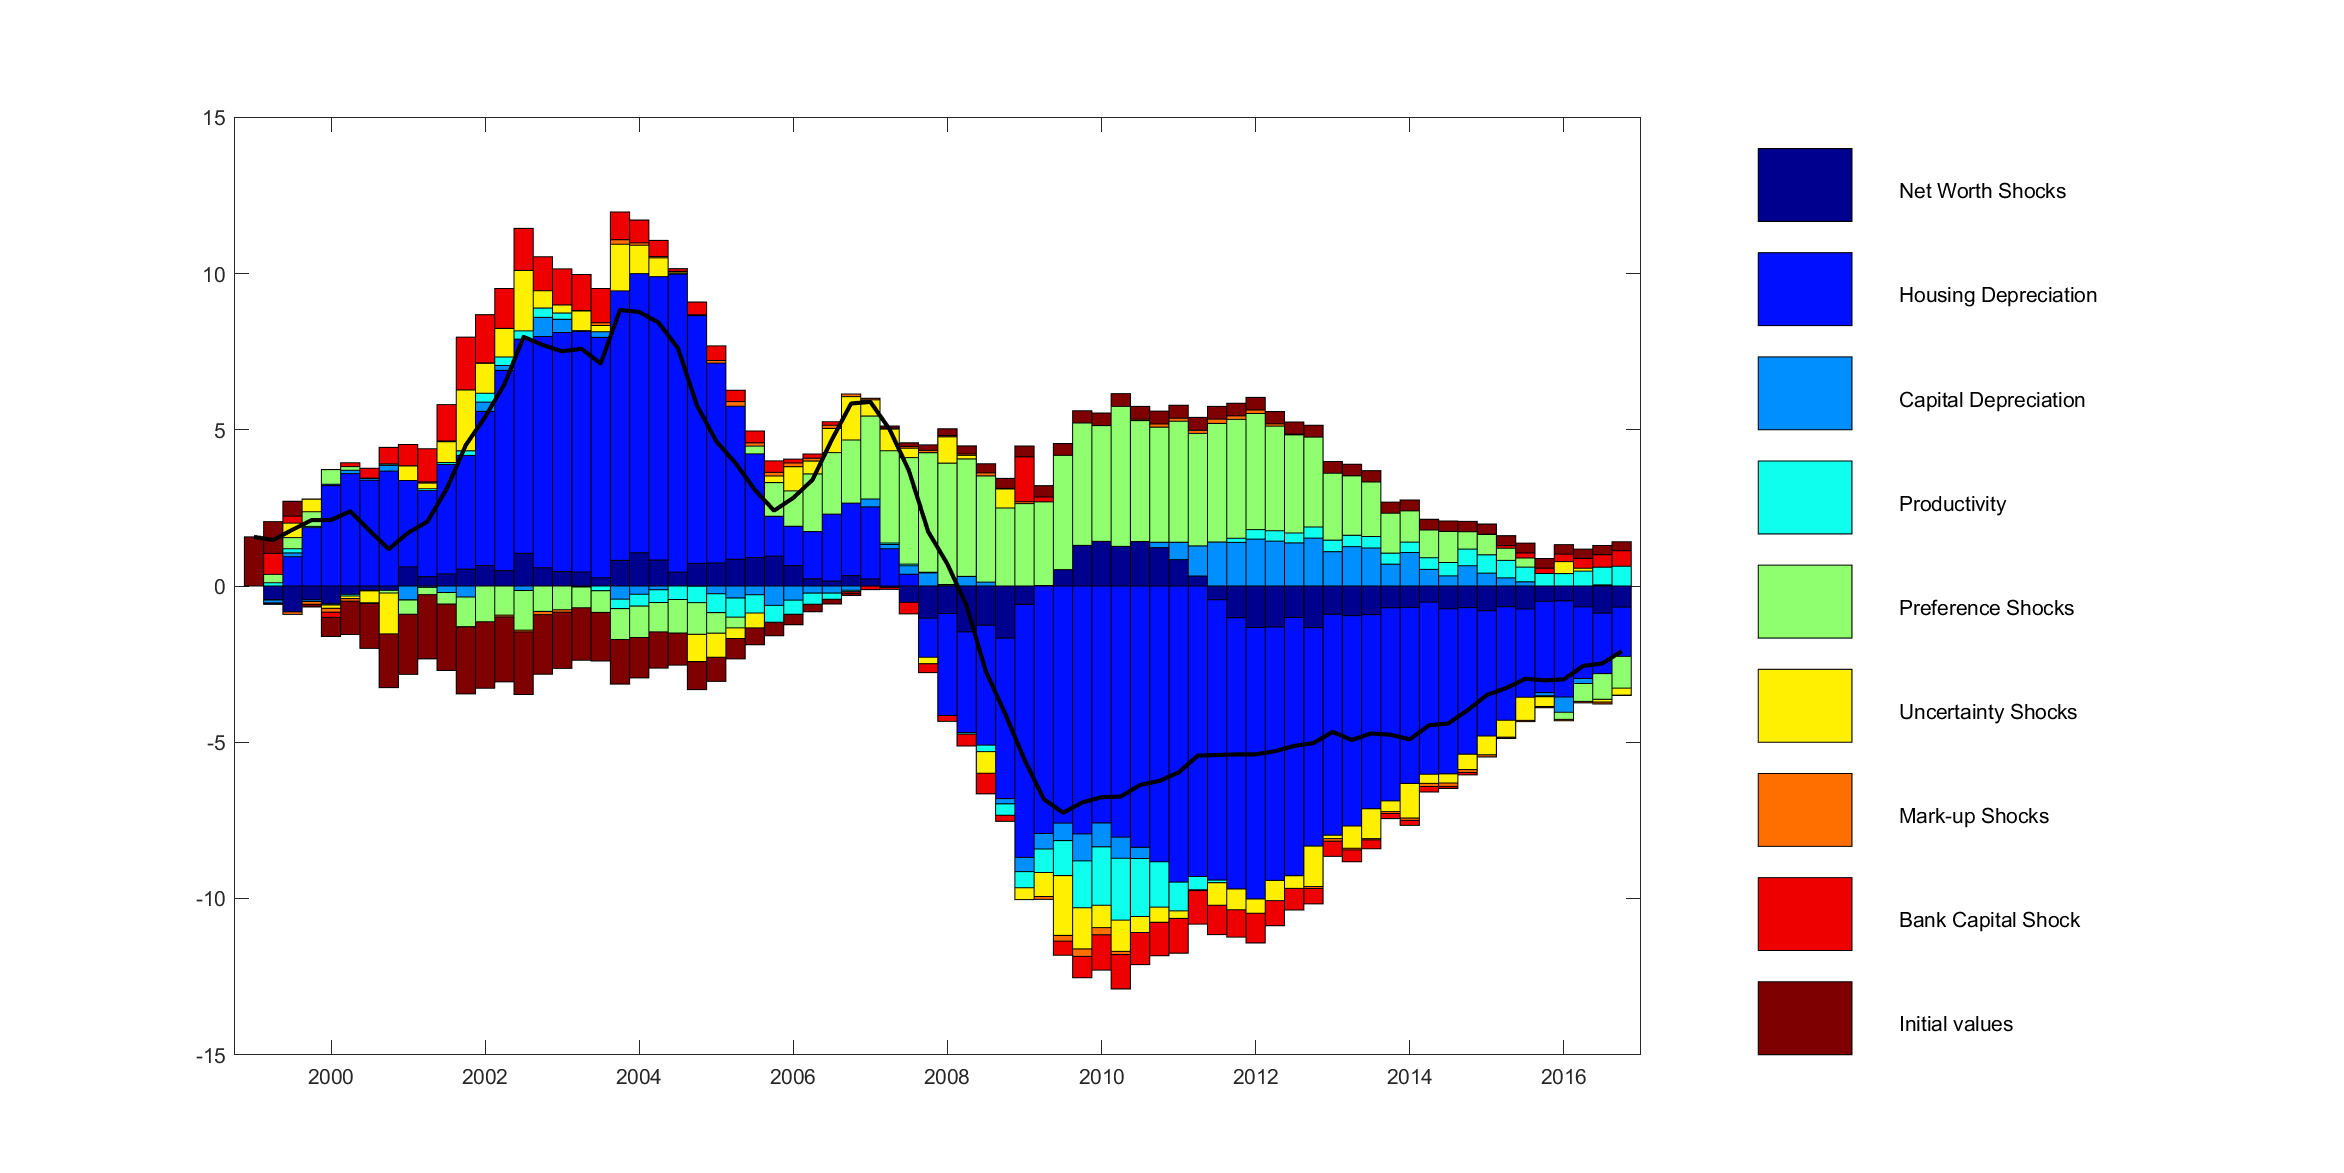
\includegraphics[scale=0.36]{decomp_dbm.pdf}
\end{figure}
\end{frame}





\begin{frame}{Estimated Shocks}

\begin{itemize}
\item What does it take in the model to generate the observed data? 

\begin{itemize}
\item Sequence of shocks over the estimation sample. 
\end{itemize}

\end{itemize}

\begin{figure}
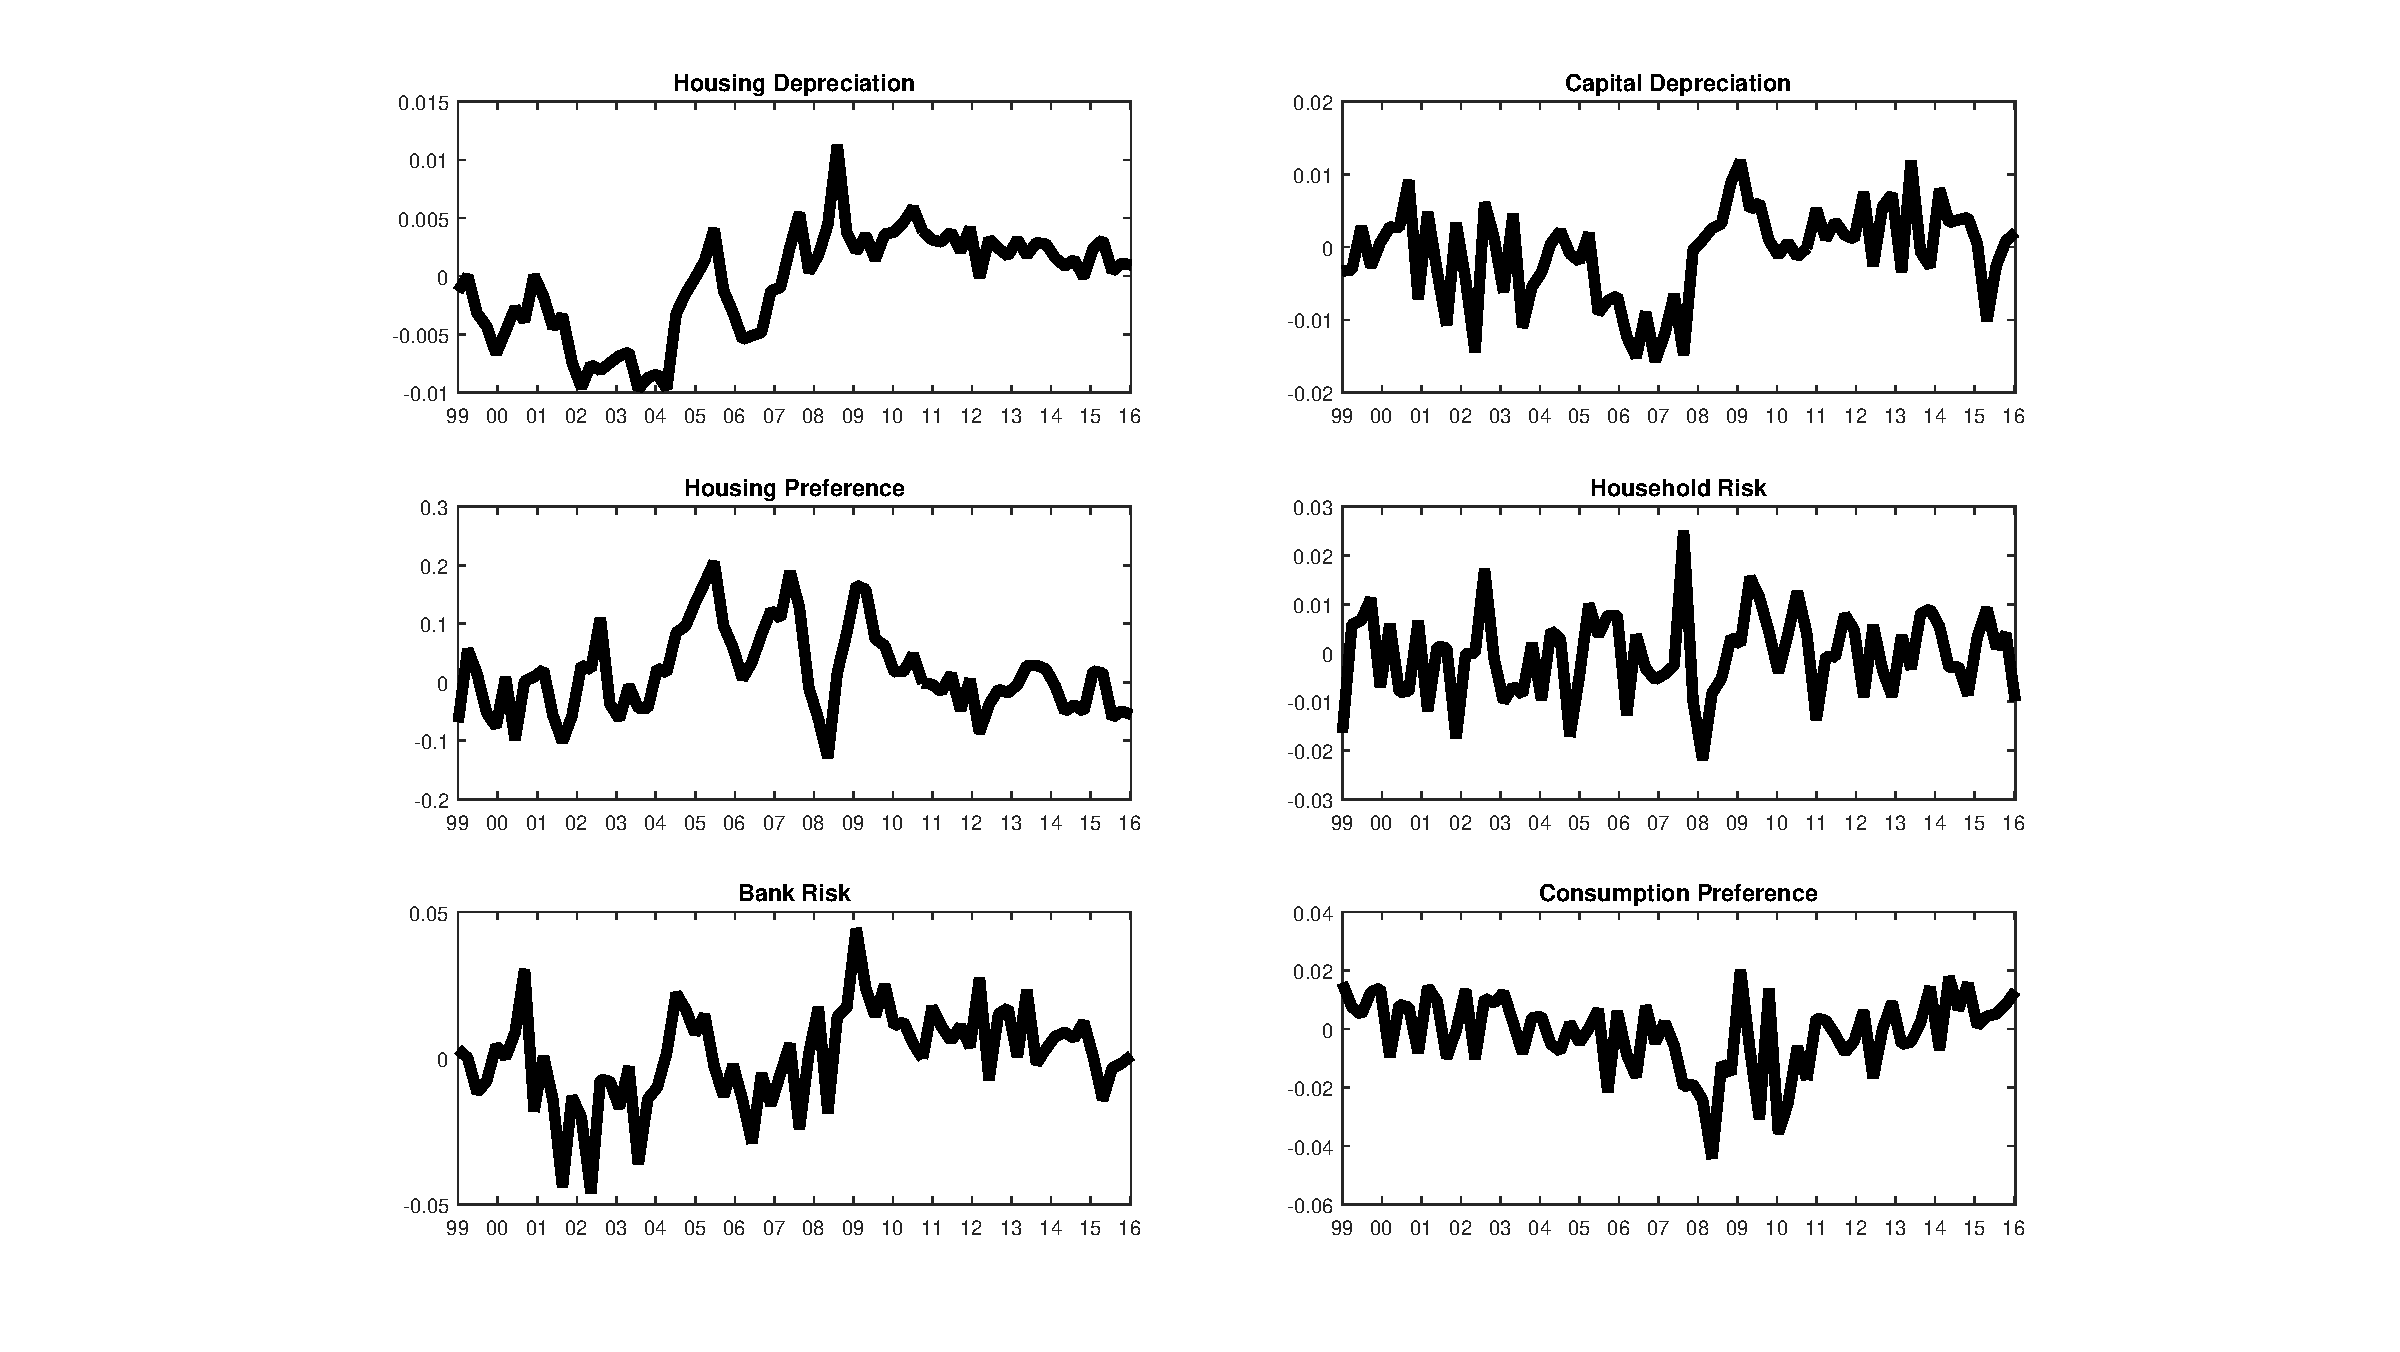
\includegraphics[scale=0.25]{smoothed_shocks.pdf}
\end{figure}
\end{frame}


\begin{frame}{Some Key Unobservables}



\begin{figure}
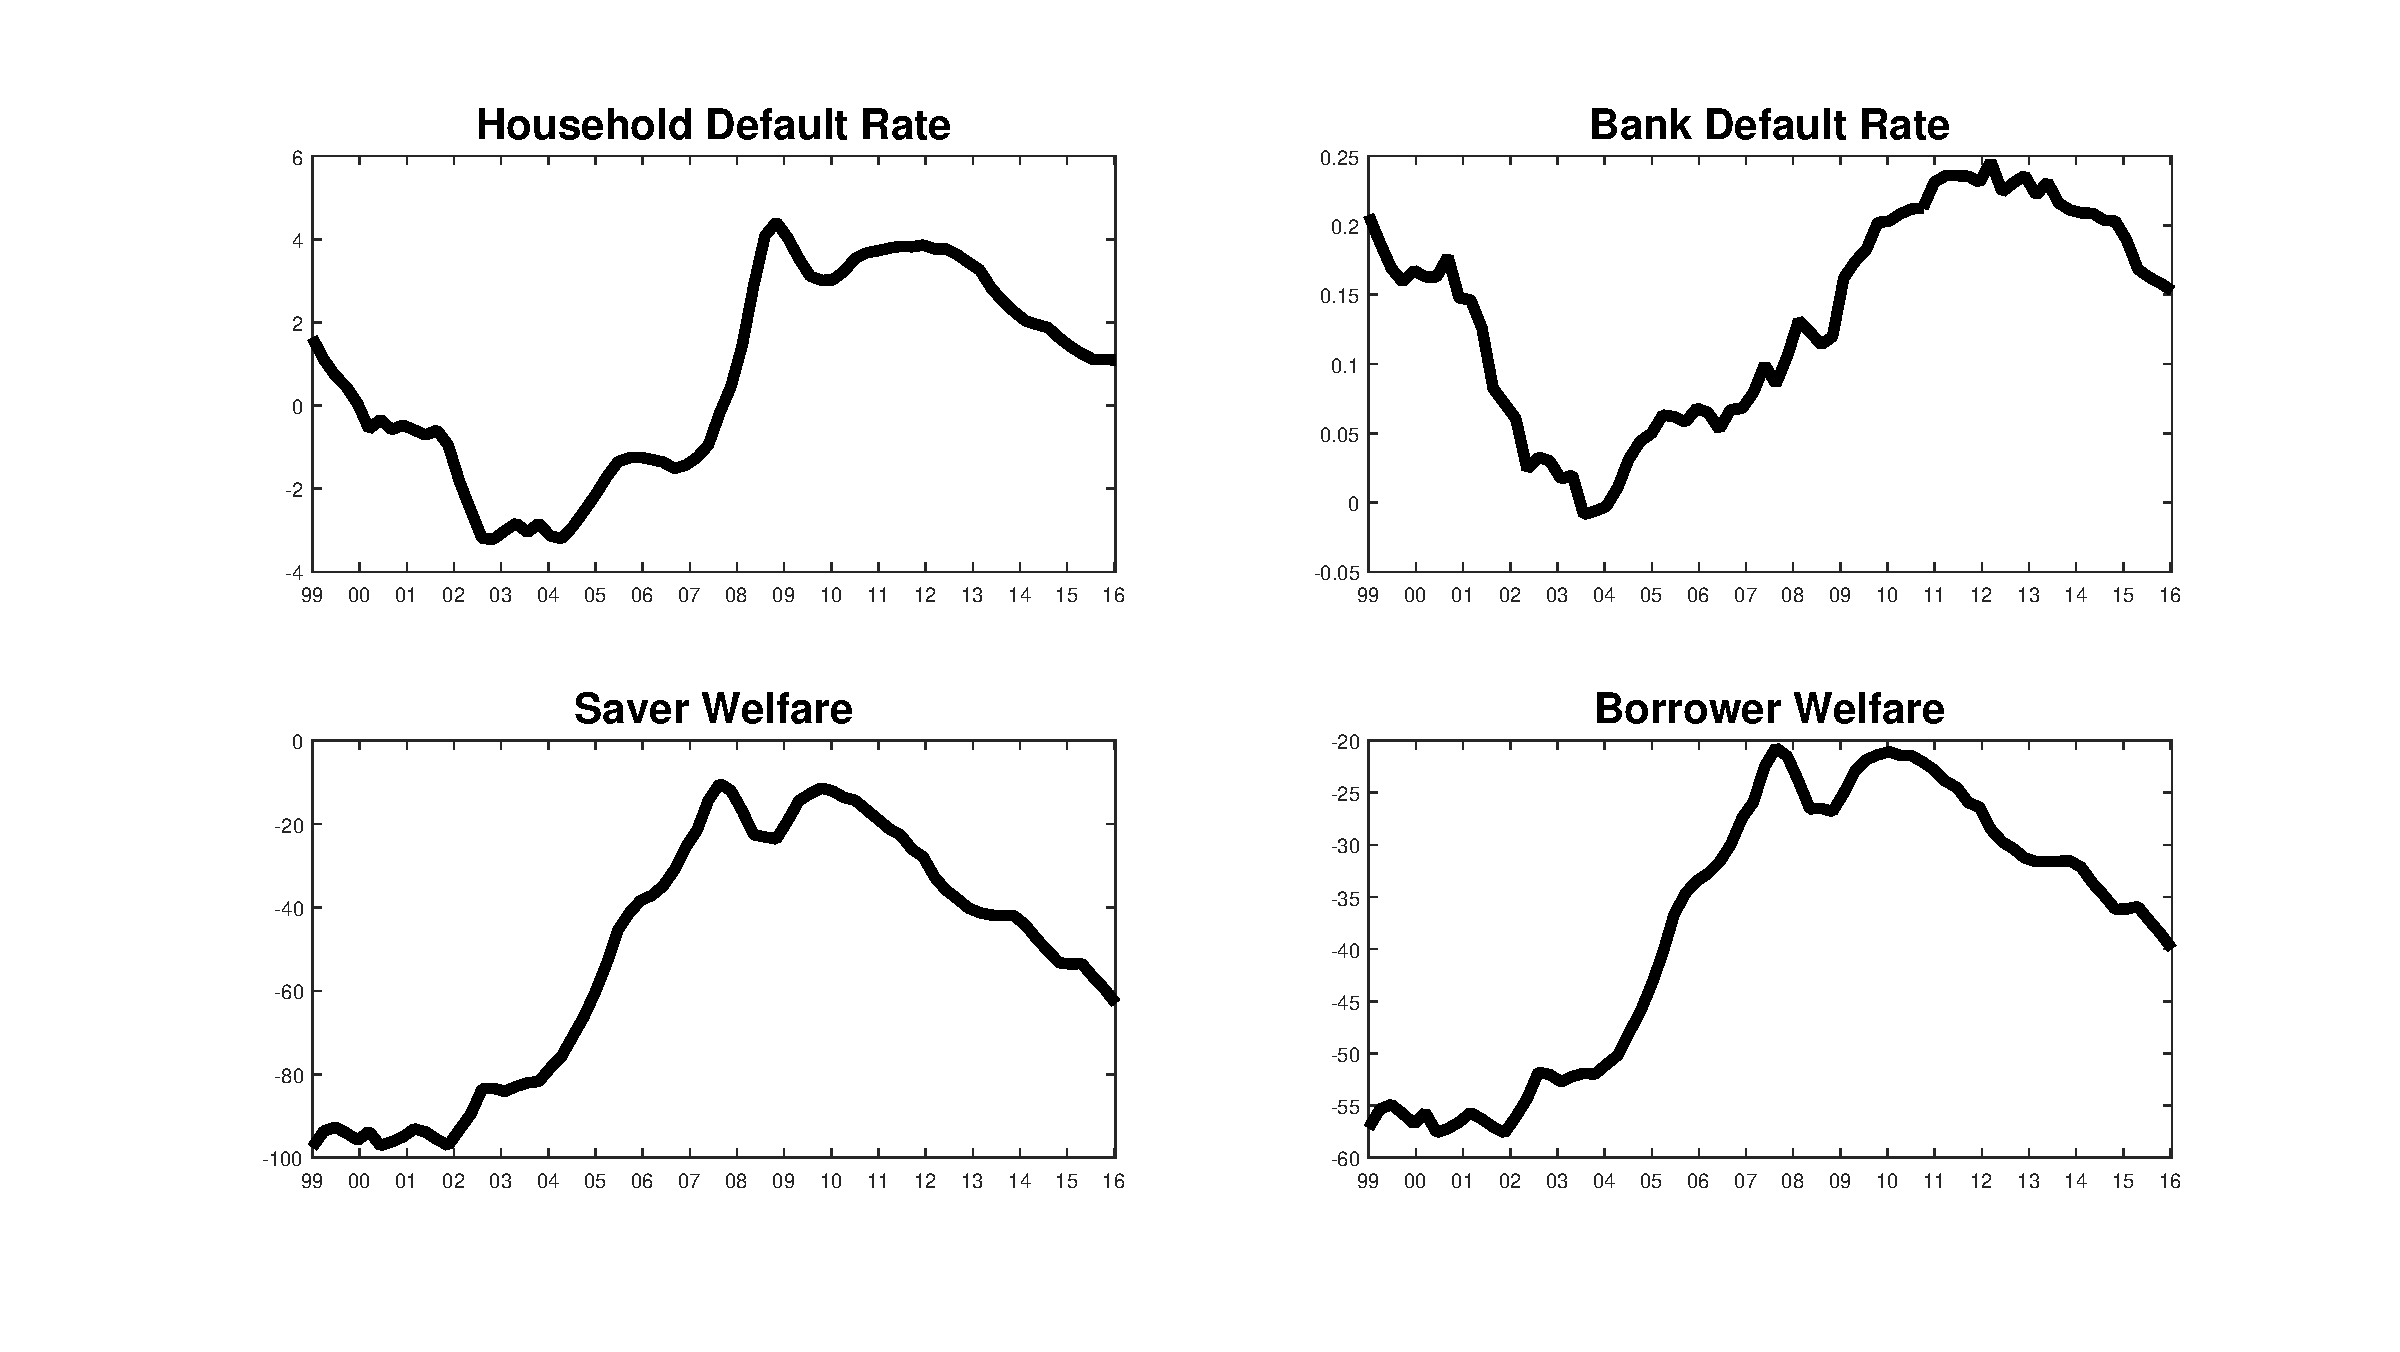
\includegraphics[scale=0.25]{smoothed_variables.pdf}
\end{figure}


\end{frame}



\begin{frame}{Macroprudential Policy}

\begin{itemize}

\item Available tools in the model: 
\vspace{3 mm}
\begin{itemize}
\item Minimum and sectoral capital requirements (Benchmark: 11 \%)
\vspace{3 mm}
\item LTV limit on businesses and households (Benchmark: 86 \%)
\vspace{3 mm}
\item CCyB (Benchmark: 0)
\end{itemize}
\vspace{5 mm}
\item Steady-state welfare analysis
\vspace{5 mm}
\item Shock propagation and counterfactuals
\vspace{5 mm}
\item Prudential policy \& Imperfect interest-rate pass through

\end{itemize}
\end{frame}



\begin{frame}{Minimum Capital Requirements and Steady-state}

\begin{figure}[H]
\centering
%\caption{Sectoral capital requirements on mortgage lending with a baseline of 11 \%. Welfare maximizing value is 20.7 \% with a weight of 0 on volatility. It decreases to 17.6 \% with a weight of 0.1 on the volatility.
%\textbf{Welfare improvement: 7.47 \% and 4.26 \% respectively.} } 
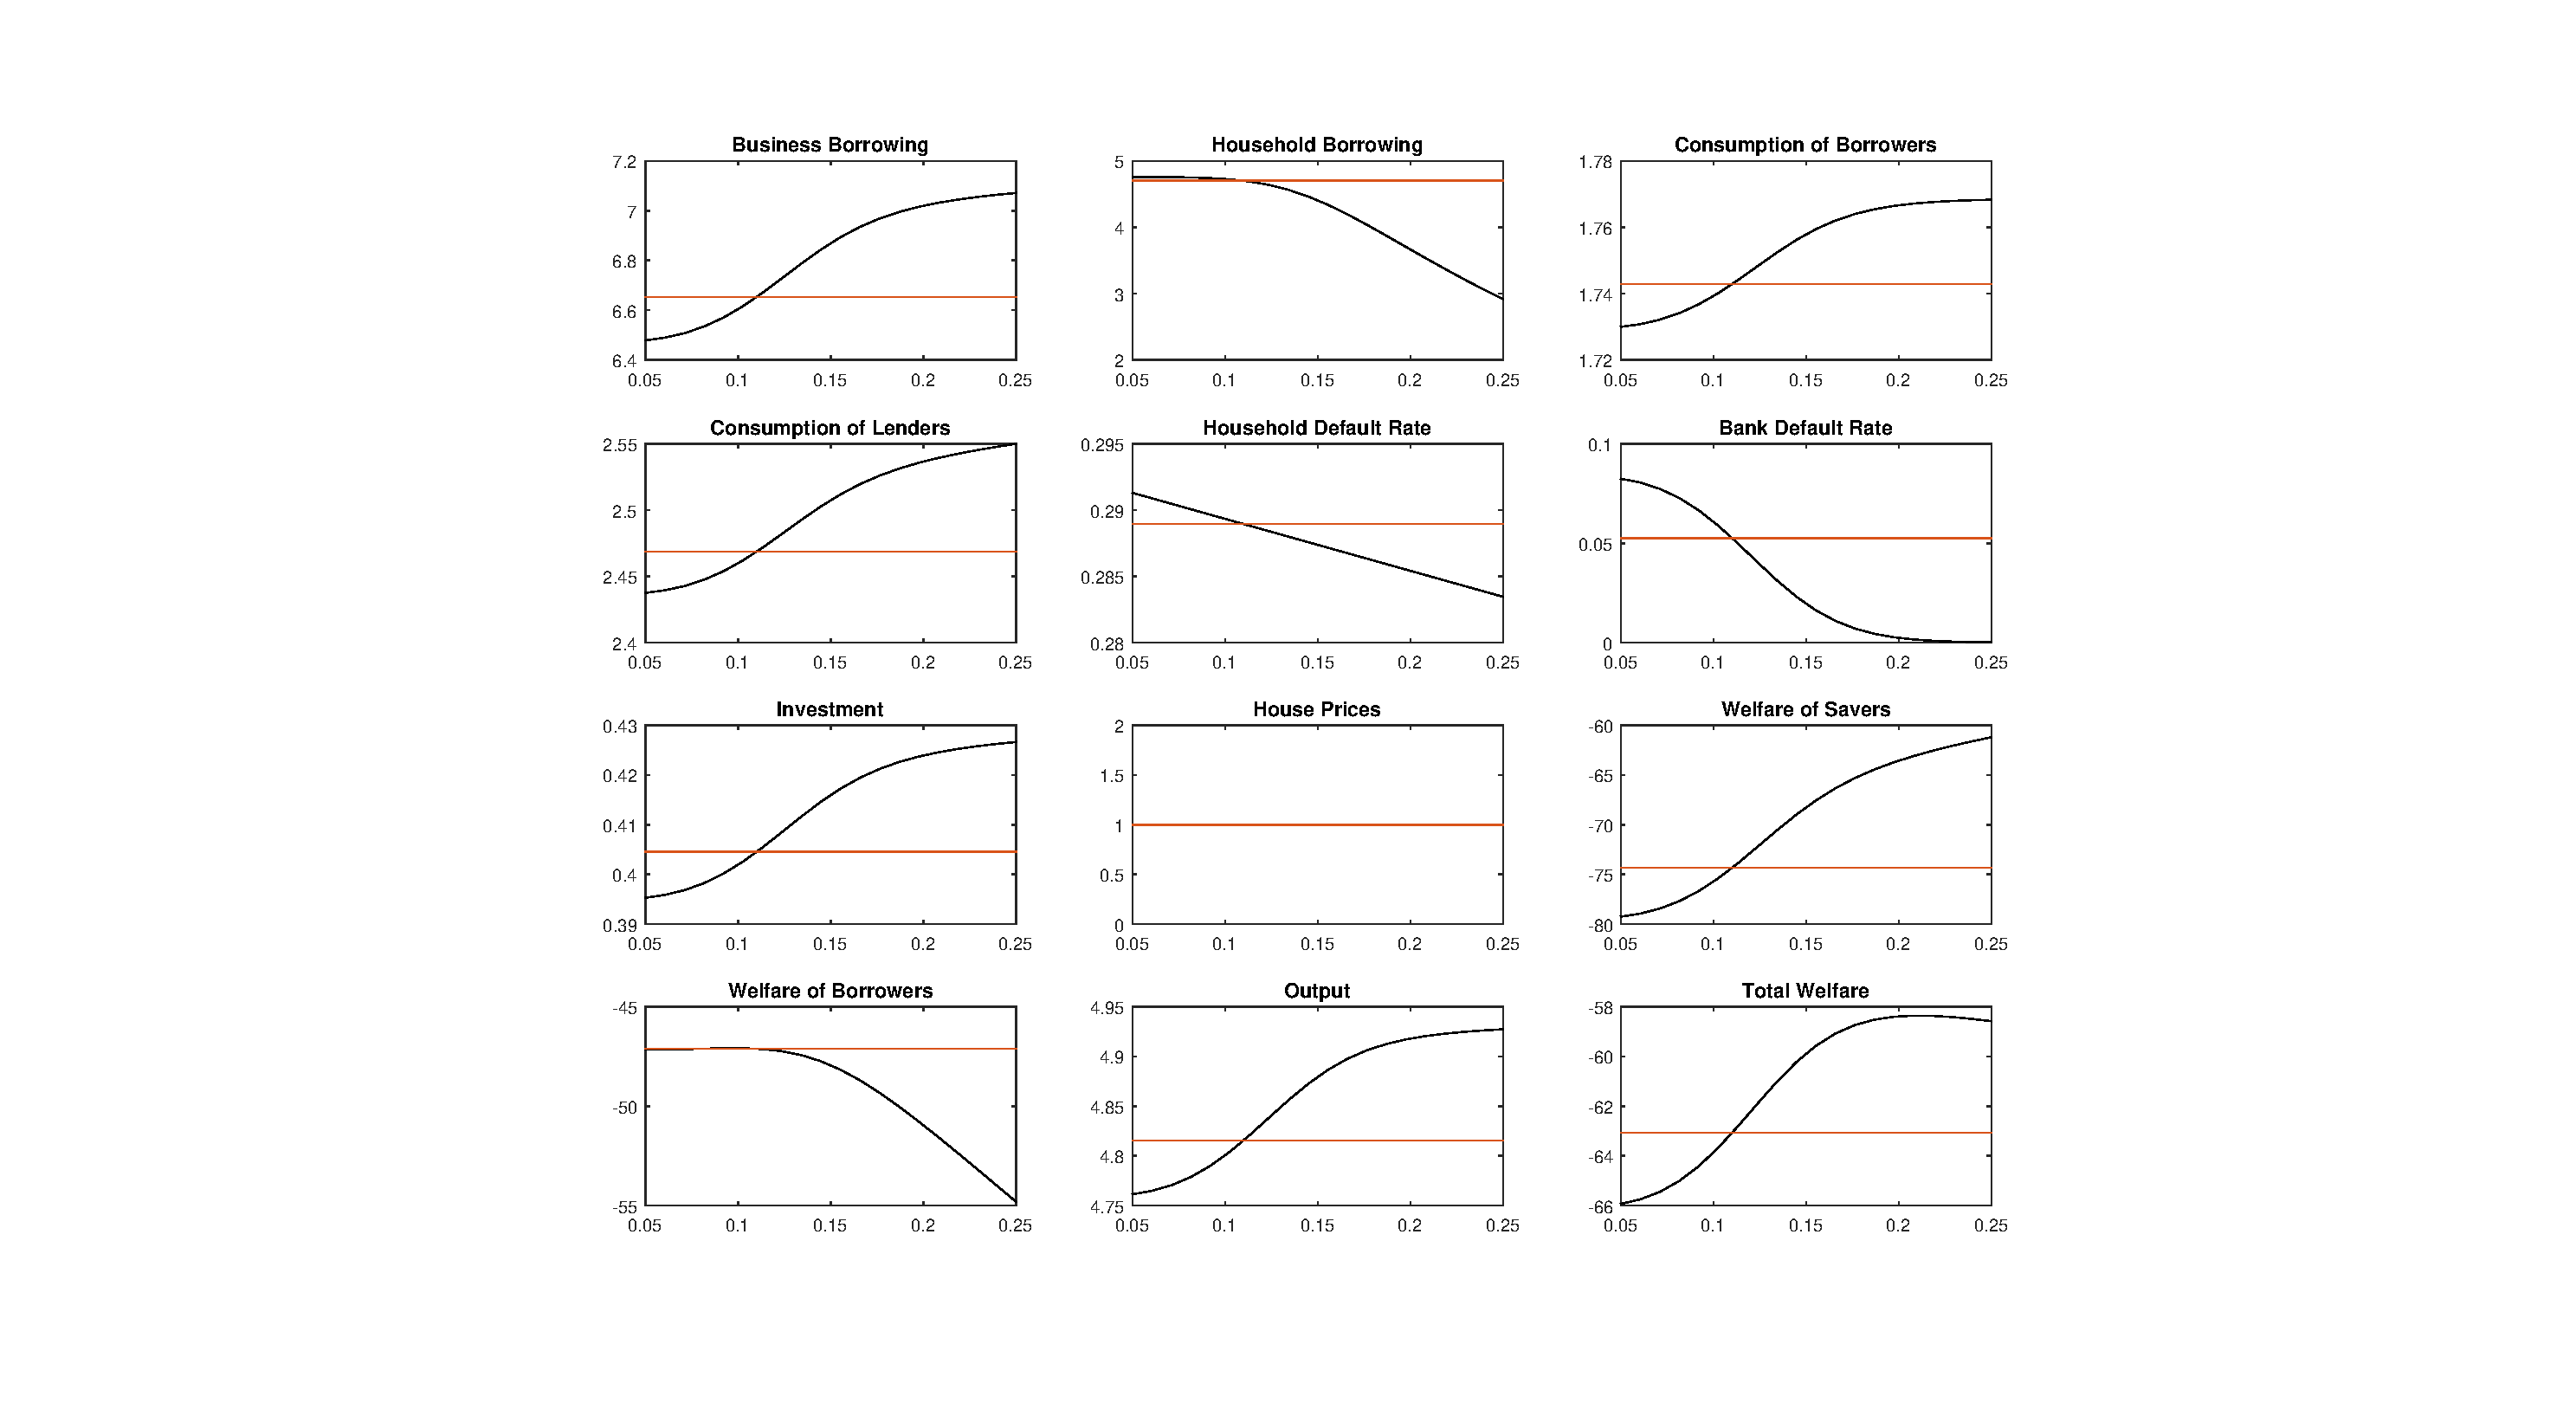
\includegraphics[scale=0.3]{WA2_level.pdf}\\

\end{figure}

\end{frame}


\begin{frame}{Minimum Capital Requirements and Volatility}

\begin{figure}[H]
\centering
%\caption{Sectoral capital requirements on mortgage lending with a baseline of 11 \%. Welfare maximizing value is 20.7 \% with a weight of 0 on volatility. It decreases to 17.6 \% with a weight of 0.1 on the volatility.
%\textbf{Welfare improvement: 7.47 \% and 4.26 \% respectively.} } 
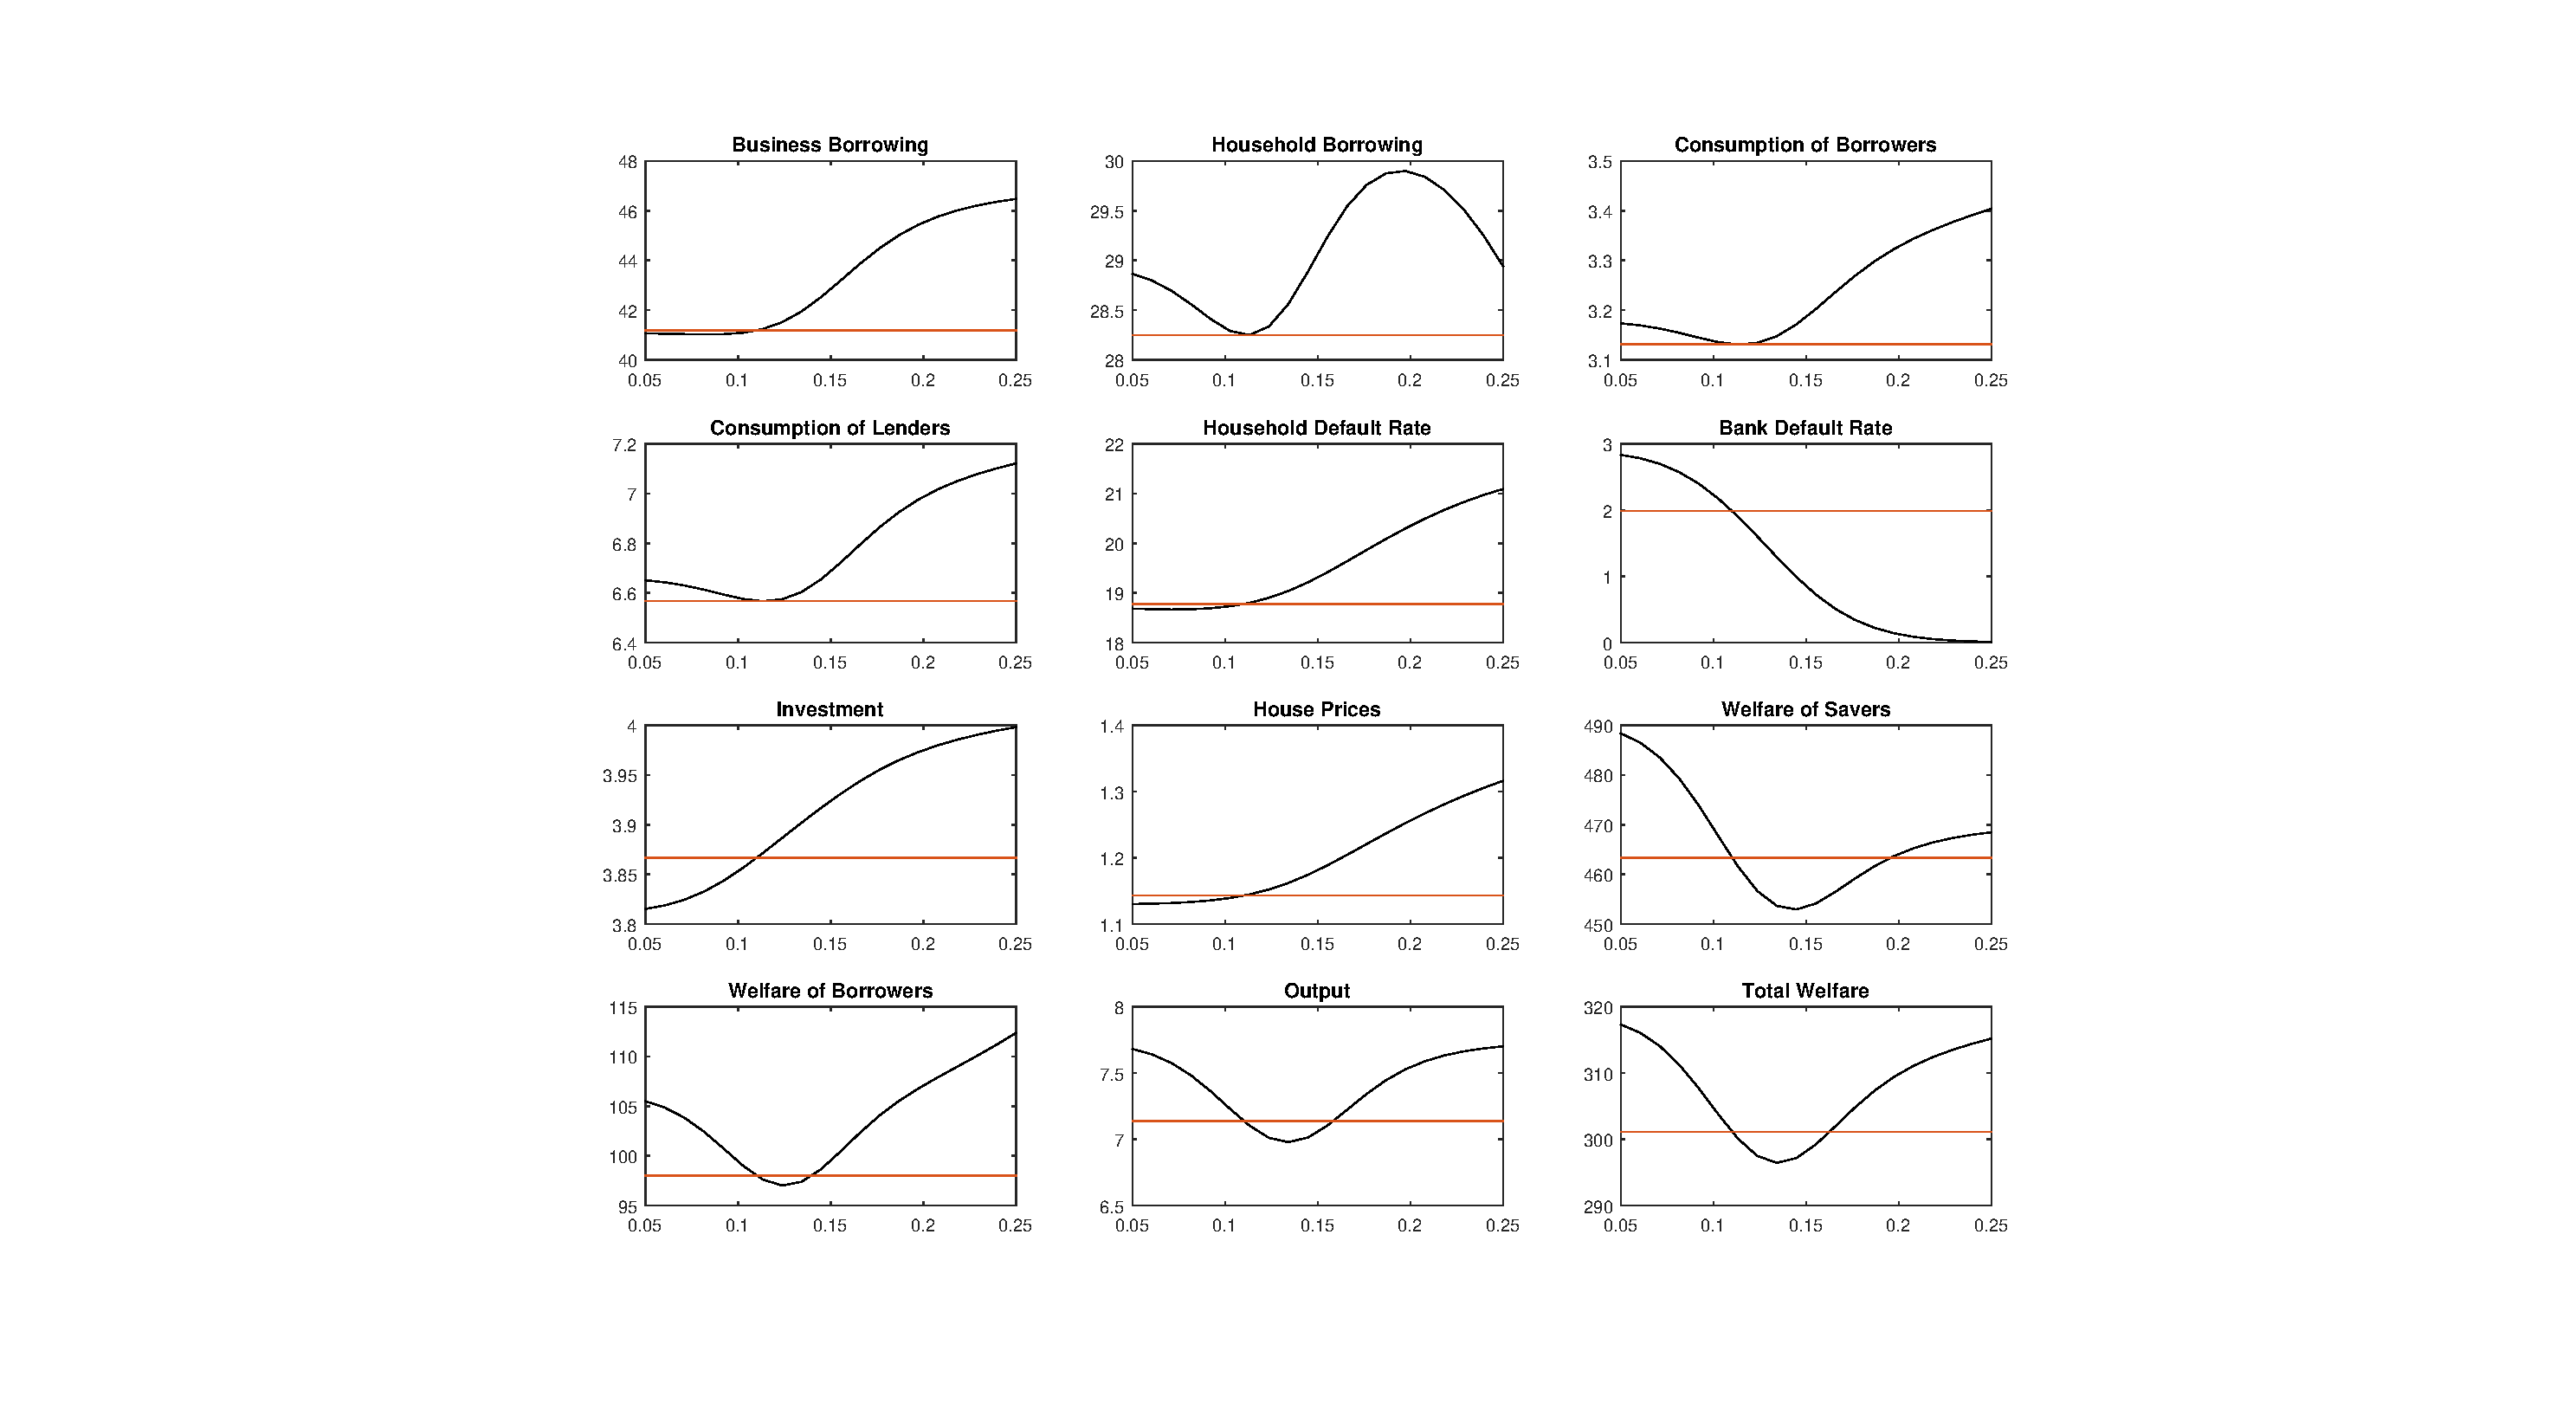
\includegraphics[scale=0.3]{WA2_var.pdf}
\end{figure}

\end{frame}



\begin{frame}{Optimal Policies}

\begin{itemize}
\item Ad-hoc objective function: $  E[W_t] - \omega \sqrt{Var[W_t]}  $
\end{itemize}

\begin{table}[h]

\caption{Maximizing over prudential policy parameters, one at a time.}
\begin{tabular}{l|l|l|l}

 & $\omega$ & 0 & 0.1   \\
 \hline
 \hline
Parameter & & &  \\
\hline
\hline
LTV &  & 89.4 \% (0.014 \%) & 86.6 \% (0.001 \%)  \\

SCR-Mortgage &  & 20.7 \% (7.47 \%) & 17.6 \% (4.26 \%) \\

SCR-Corporate & & 15.5 \% (3.33 \%) & 16.7 \% (3.22 \%) \\

CAR & & 15.5 \% (5.11 \%) & 14.5 \% (3.82 \%) \\

CCyB & & 0 \% (0 \%) & Max. attainable \\

\end{tabular}
\end{table}



\begin{table}[h]

\caption{Optimal joint SCRs and LTV}
\begin{tabular}{l|l|l|l}

 & $\omega$ & 0 & 0.1   \\
 \hline
 \hline
Parameter & & &  \\
\hline
\hline
LTV &  & 91.25 \%   &  94.06 \%  \\

SCR-Mortgage &  & 21.25 \%     & 15.88 \%   \\

SCR-Corporate & &  5(Min. attainable) \%  & 12.50 \%  \\

Welfare Improvement & & 8.01 \% & 4.8 \% \\

\end{tabular}
\end{table}



\end{frame}



\begin{frame}{Counterfactual I}
\begin{figure}[H]
\centering
\caption{Counterfactual I: using optimized values  with 0.1 weight on volatility. $\phi_H=15.8 \%, \phi_F=12.5 \%, \epsilon_H=94 \%$.}
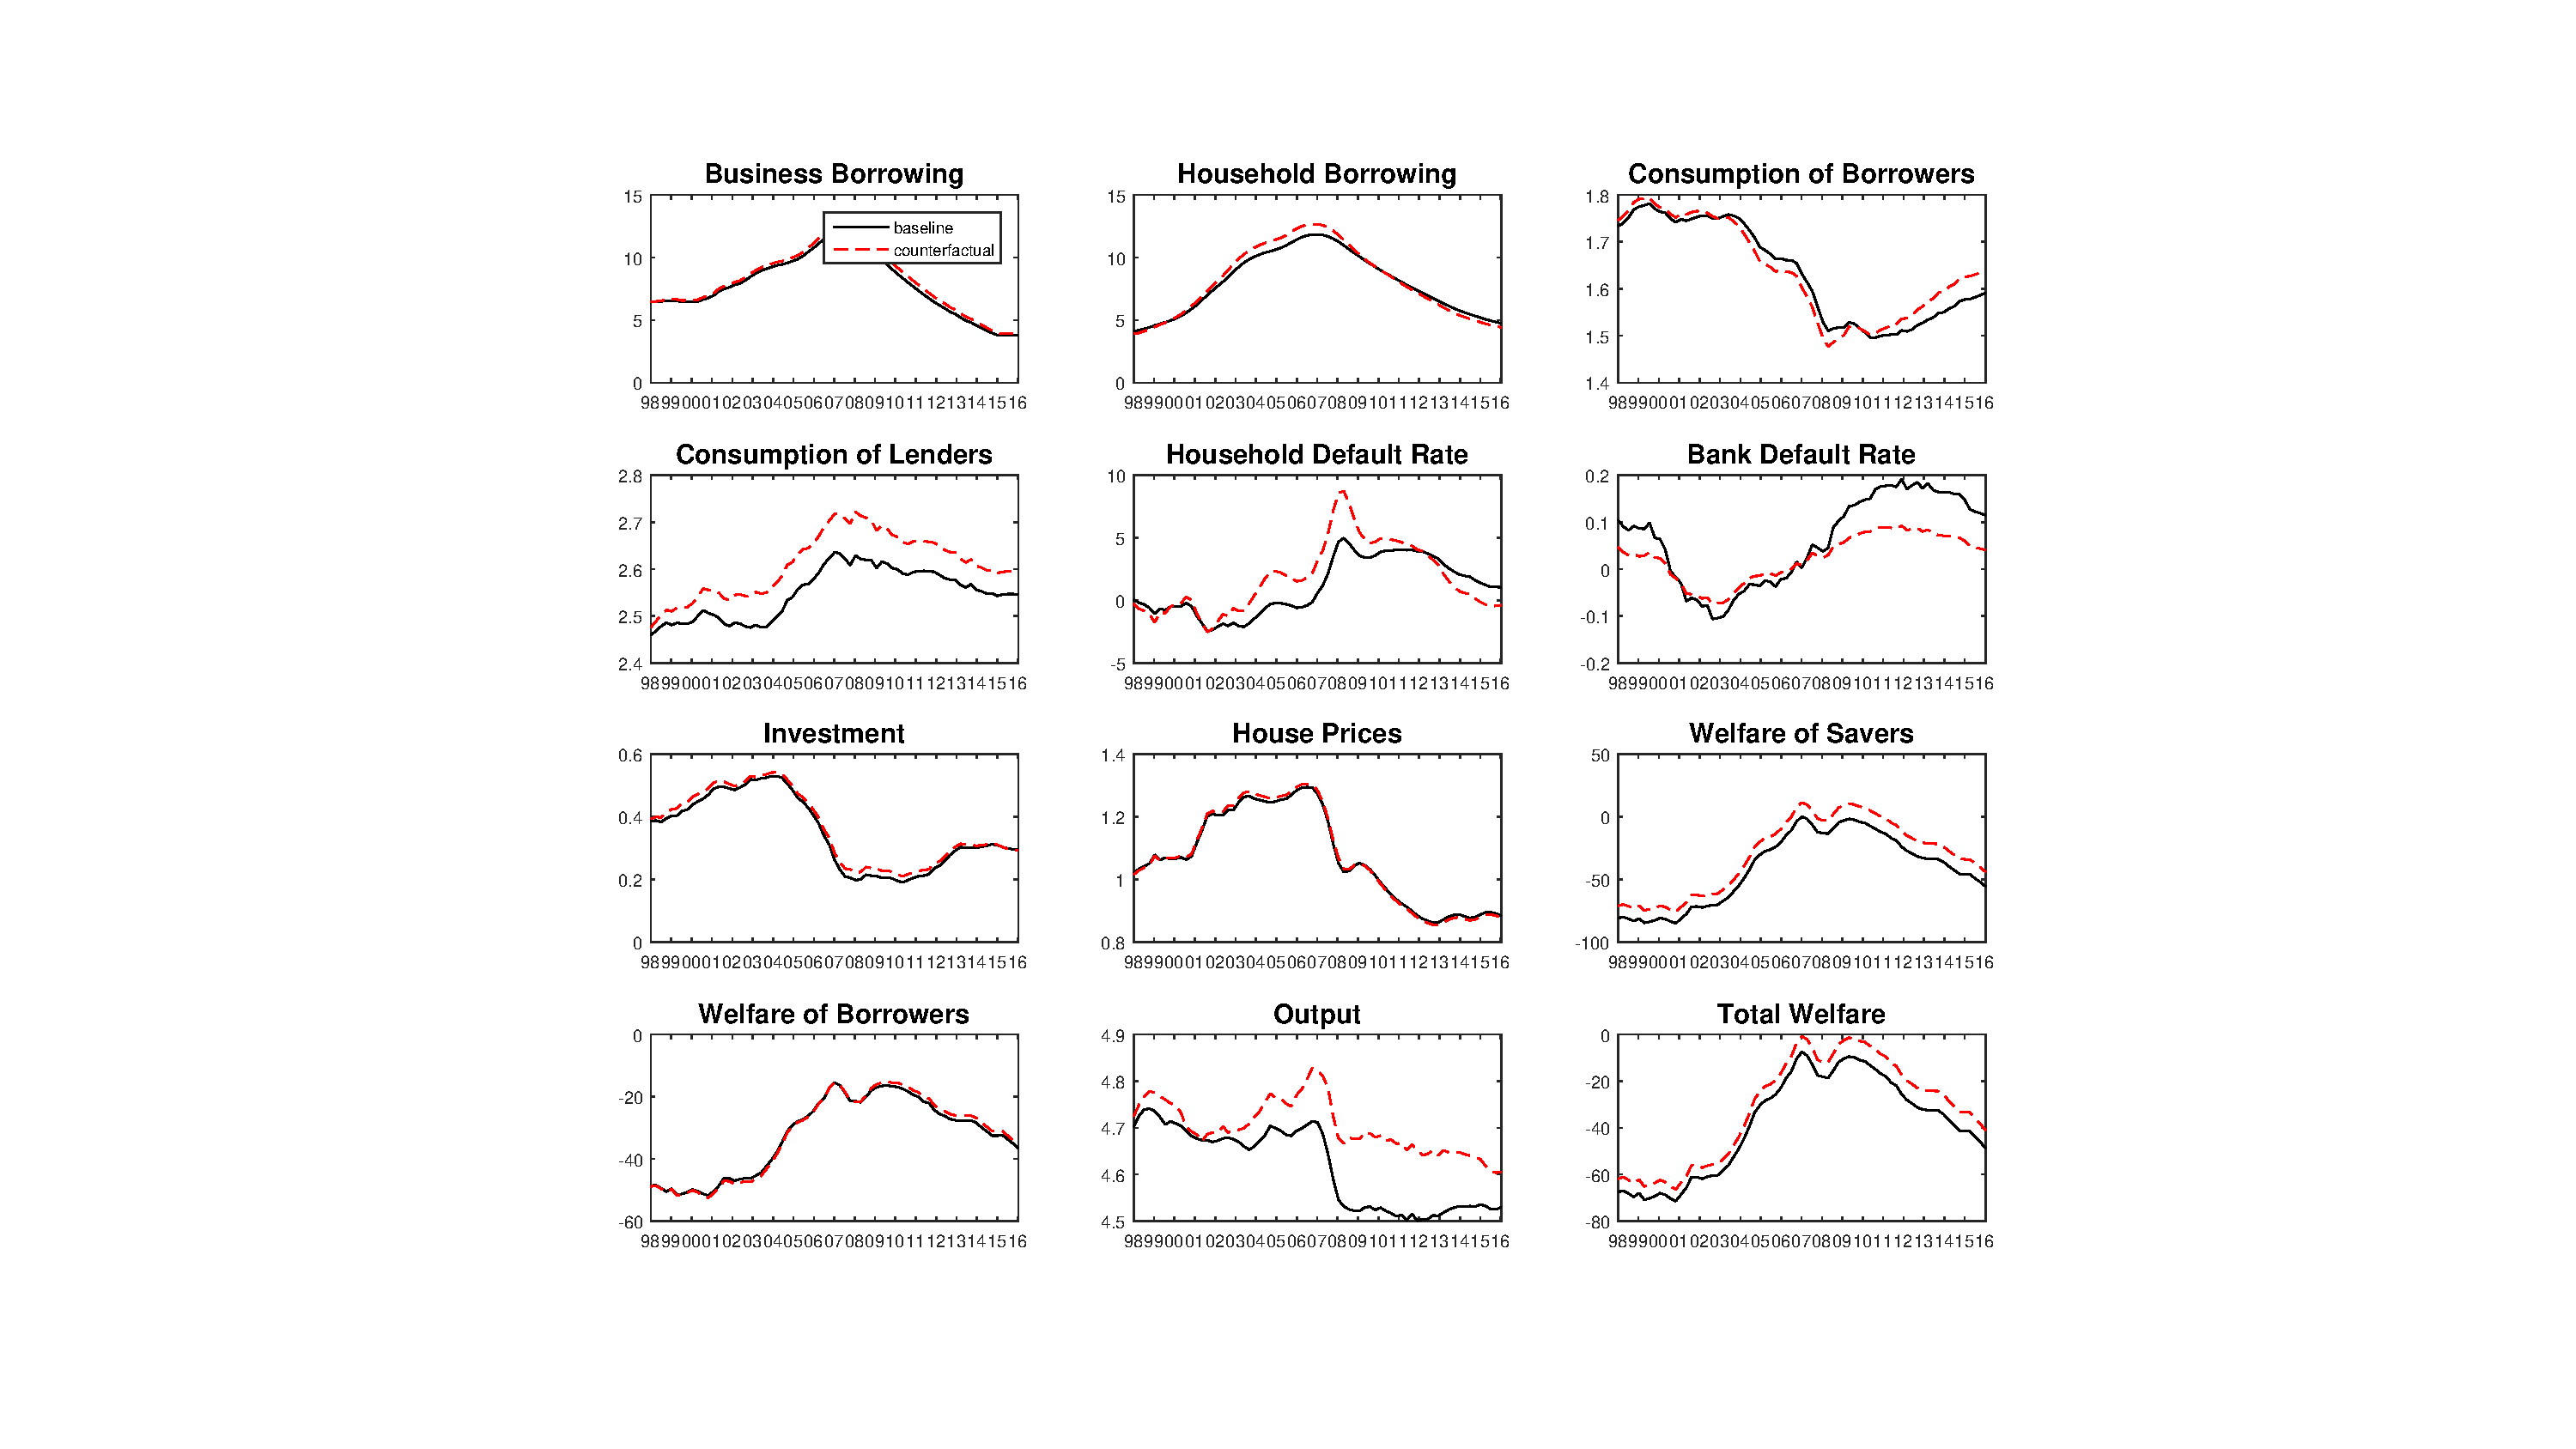
\includegraphics[scale=0.25]{counterfactuals2.pdf}
\end{figure}
\end{frame}




\begin{frame}{Changes in the Level and Volatility}

\begin{table}[h]

\begin{tabular}{l|l|l}
Variable & \% Change in Level & \% Change in Volatility \\
\hline
\hline
    Corporate Credit           &       0.039    &      0.041 \\
    Mortgage Credit            &      0.024    &       0.147 \\
    Output         &     0.019    &    -0.354 \\ 
    Household Welfare       &     0.175     &     0.0437\\
\end{tabular}
\end{table}


\end{frame}



\begin{frame}{Counterfactual II: Phasing-in}



\begin{figure}[H]
\centering
\caption{Same counterfactual phased-in over a 5-year period over 2001-2006 in equal increments.}
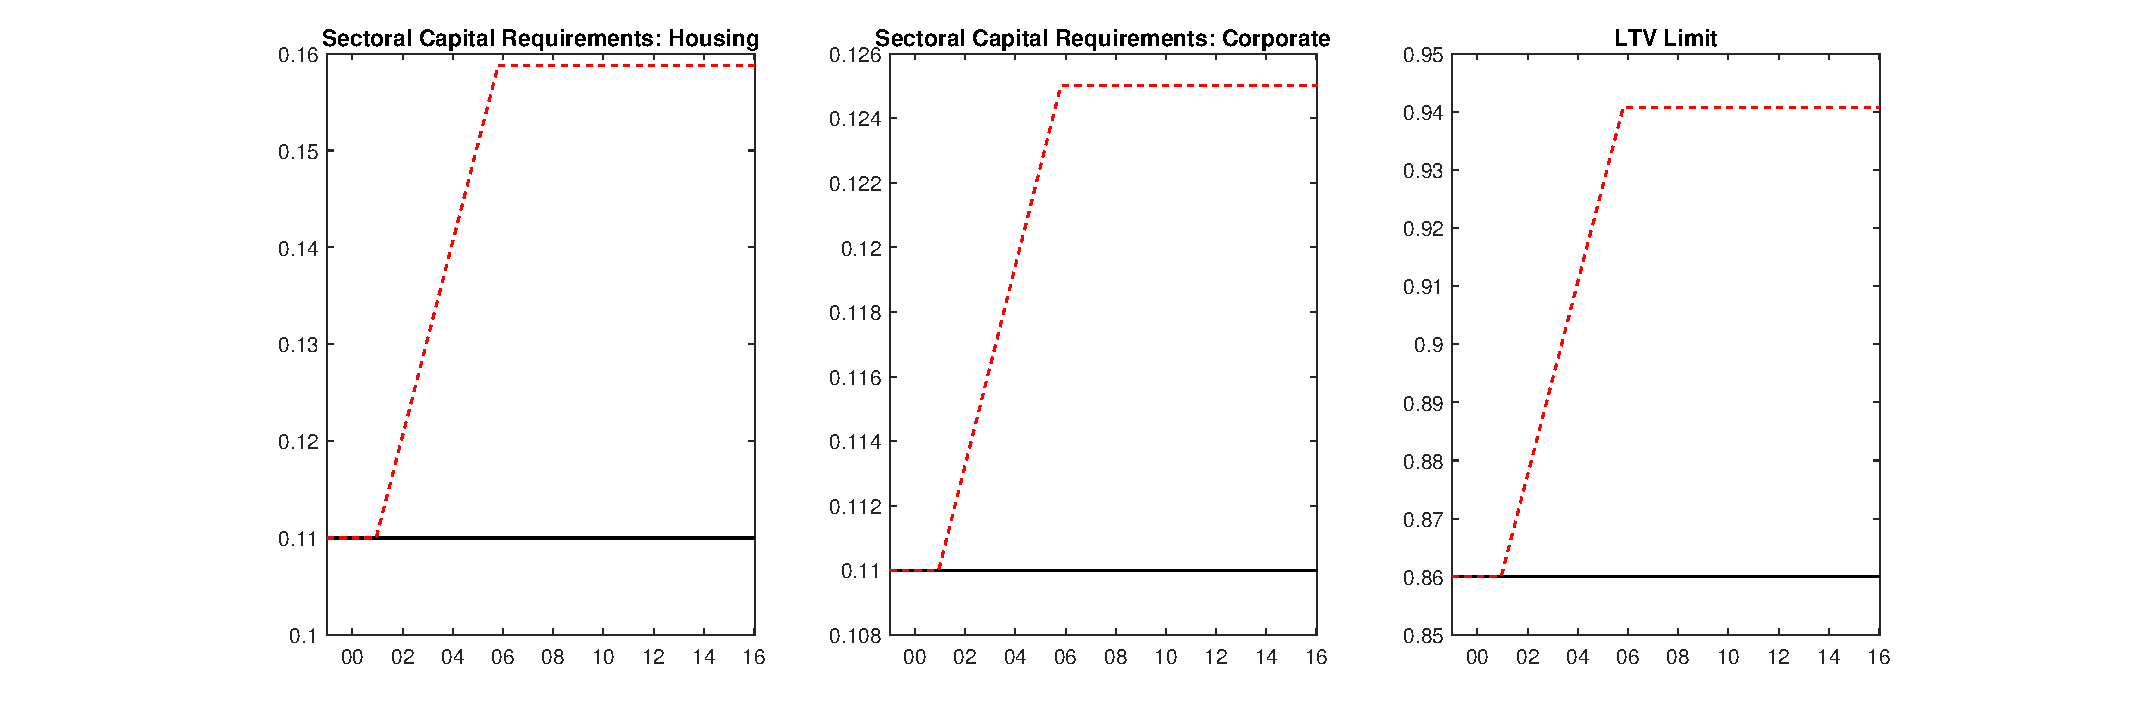
\includegraphics[scale=0.35]{CF_policy_rules10.pdf}
%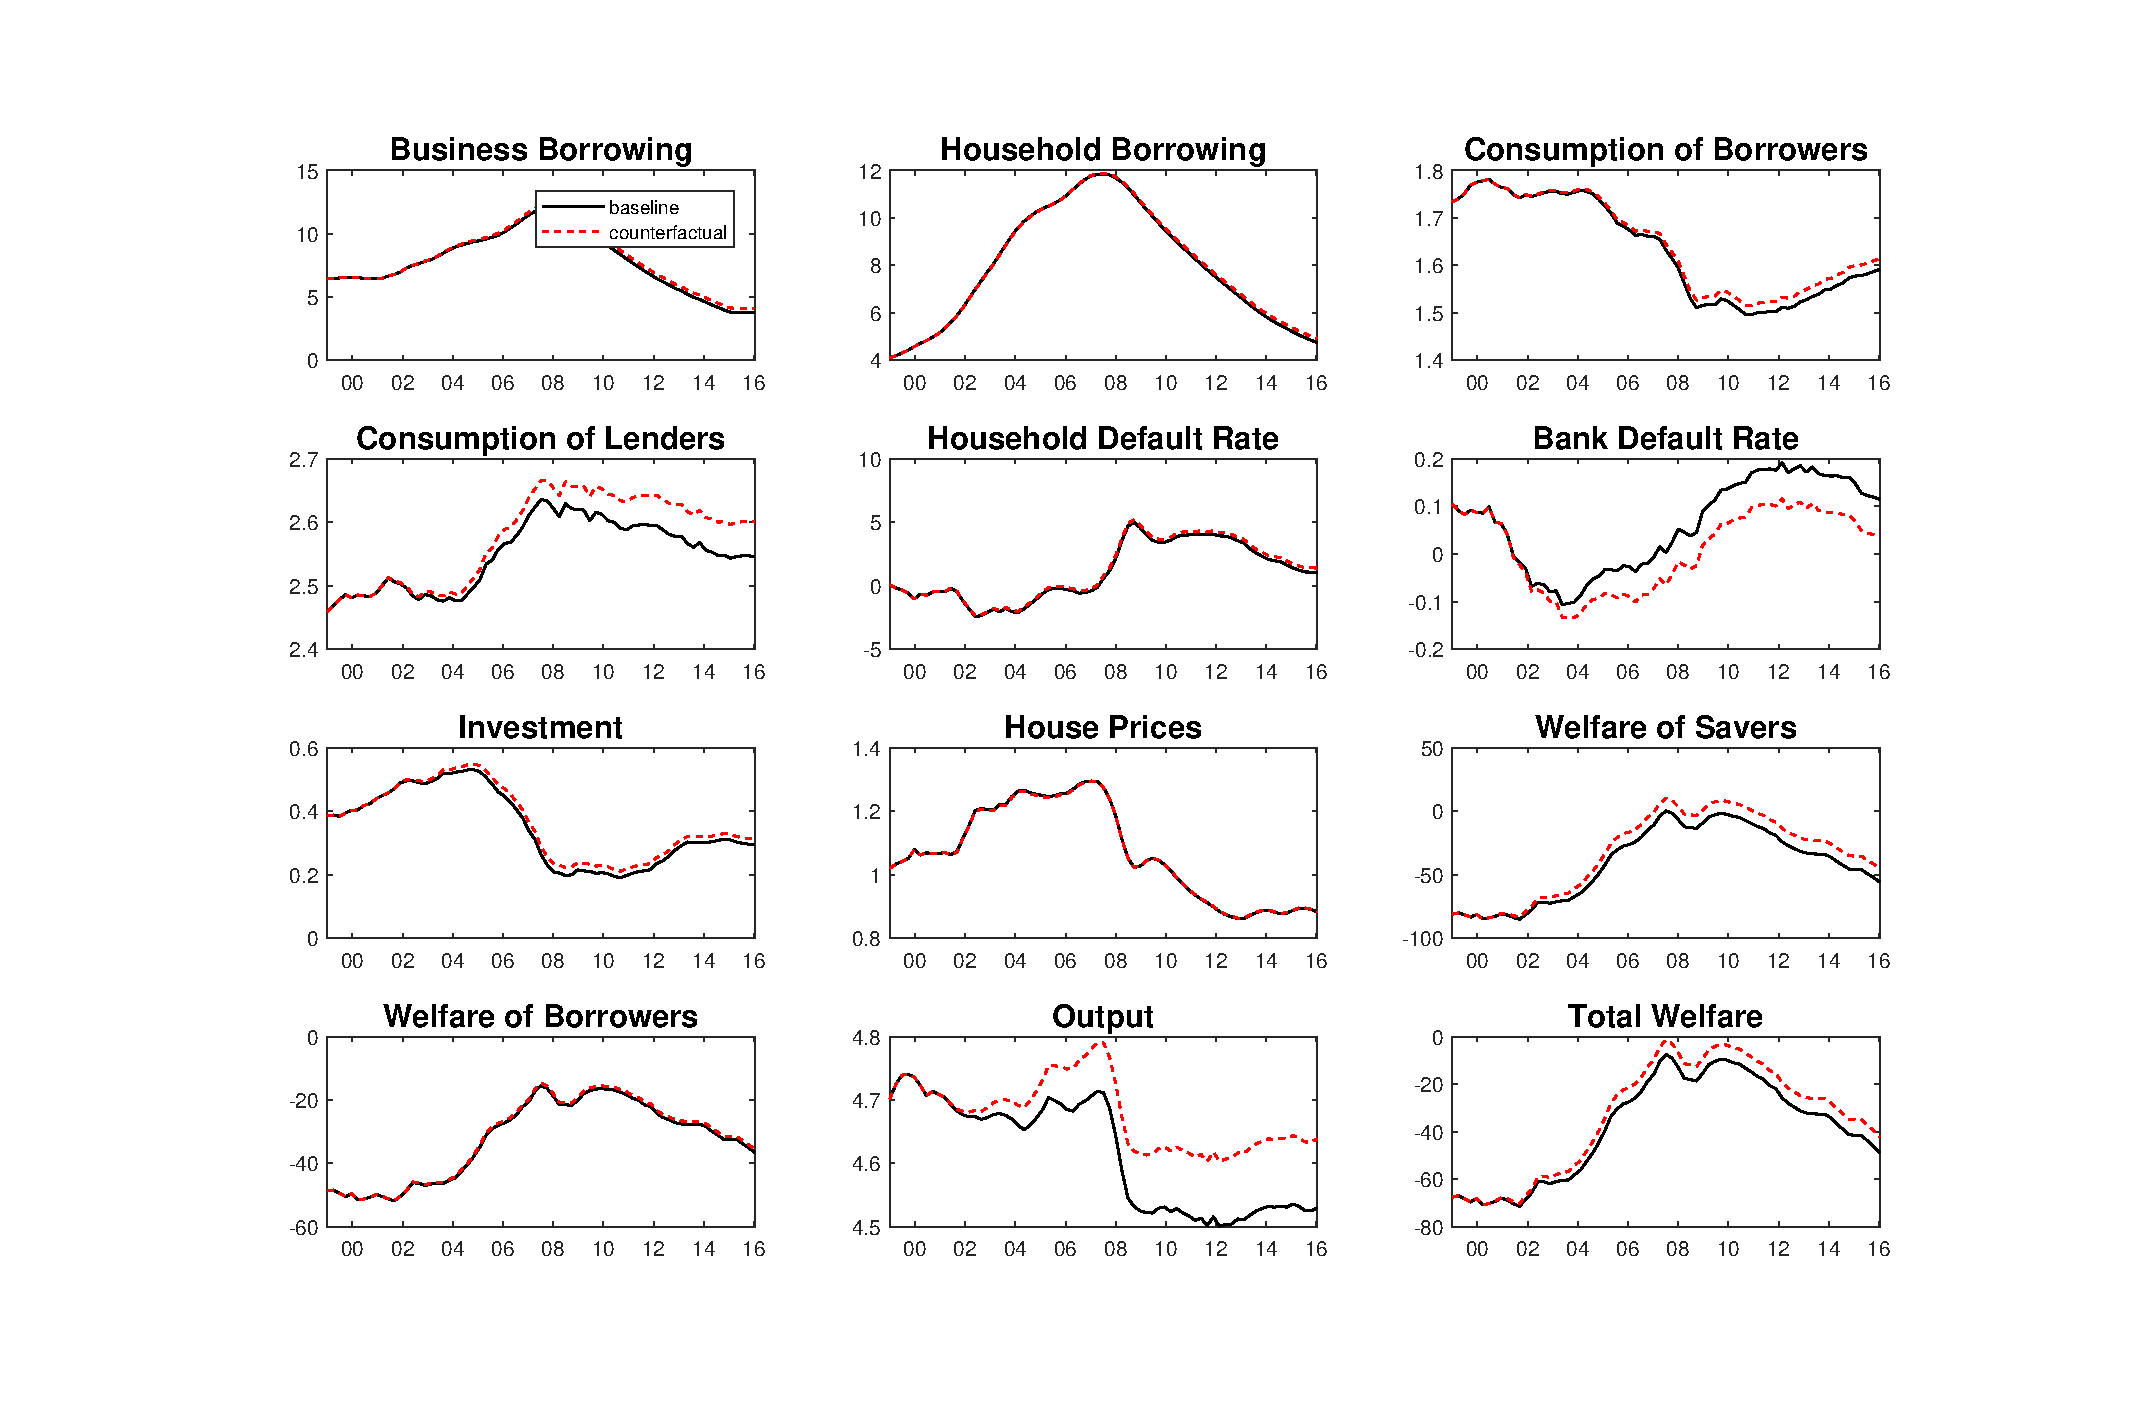
\includegraphics[scale=0.45]{counterfactuals10.pdf}\\

\end{figure}


\end{frame}


\begin{frame}{Changes in the Level and Volatility}

\begin{table}[h]
\caption{Policies introduced at once at the beginning of the sample. }
\begin{tabular}{l|l|l}
Variable & \% Change in Level & \% Change in Volatility \\
\hline
\hline
    Corporate Credit           &       0.039    &      0.041 \\
    Mortgage Credit            &      0.024    &       0.147 \\
    Output         &     0.019    &    -0.354 \\ 
    Household Welfare       &     0.175     &     0.0437\\
\end{tabular}
\end{table}



\begin{table}[h]
\caption{Policies phased-in over 2001-2006.}
\begin{tabular}{l|l|l}
\small
Variable & \% Change in Level & \% Change in Volatility \\
\hline
\hline
    Corporate Credit           &       0.024    &      -0.001 \\
    Mortgage Credit            &      0.006    &       -0.007 \\
    Output         				&     0.014    &    -0.356 \\ 
    Household Welfare       &     0.12     &     0.096\\
\end{tabular}
\end{table}




\begin{table}[h]
\caption{Policies phased-in over 2001-2006, without interest rate stickiness.}
\begin{tabular}{l|l|l}
\small
Variable & \% Change in Level & \% Change in Volatility \\
\hline
\hline
    Corporate Credit           &       0.041    &     0.02 \\
    Mortgage Credit            &      0.029    &      0.08 \\
    Output         				&     0.02    &    -0.28 \\ 
    Household Welfare       &     0.12     &     0.098\\
\end{tabular}
\end{table}



\end{frame}



\begin{frame}{Introducing CCyB}

\begin{table}[h]
\caption{Does CCyB improve things when optimal SCRs are in place?}
\begin{tabular}{l|l|l}
\small
Variable & \% Change in Level & \% Change in Volatility \\
\hline
Optimal SCR+LTV & & \\
\hline
    Corporate Credit           &       0.039    &      0.041 \\
    Mortgage Credit            &      0.024    &       0.147 \\
    Output         &     0.019    &    -0.354 \\ 
    Household Welfare       &     0.175     &     0.0437\\
\end{tabular}
\end{table}



\begin{table}[h]
\caption{Does CcyB improve things when SCRs are at their baseline value? }
\begin{tabular}{l|l|l}
\small
Variable & \% Change in Level & \% Change in Volatility \\
\hline
Baseline SCR+LTV & & \\
\hline
    Corporate Credit           &       0.007    &      0.042 \\
    Mortgage Credit            &      0.003    &       0.029 \\
    Output         &     0.0019    &    0.37 \\ 
    Household Welfare       &     0.003     &     -0.002\\
  
 \hline
No Interest Stickiness & & \\
\hline

    Corporate Credit           &       0.016    &      0.072 \\
    Mortgage Credit            &      0.008    &       0.108 \\
    Output         &     0.005    &    0.675 \\ 
    Household Welfare       &     0.013     &     -0.009\\
  \end{tabular}
\end{table}


\end{frame}





\begin{frame}{Interest-rate Stickiness on Shock Propagation-I}



\begin{figure}[H]
\centering
\caption{TFP Shock}
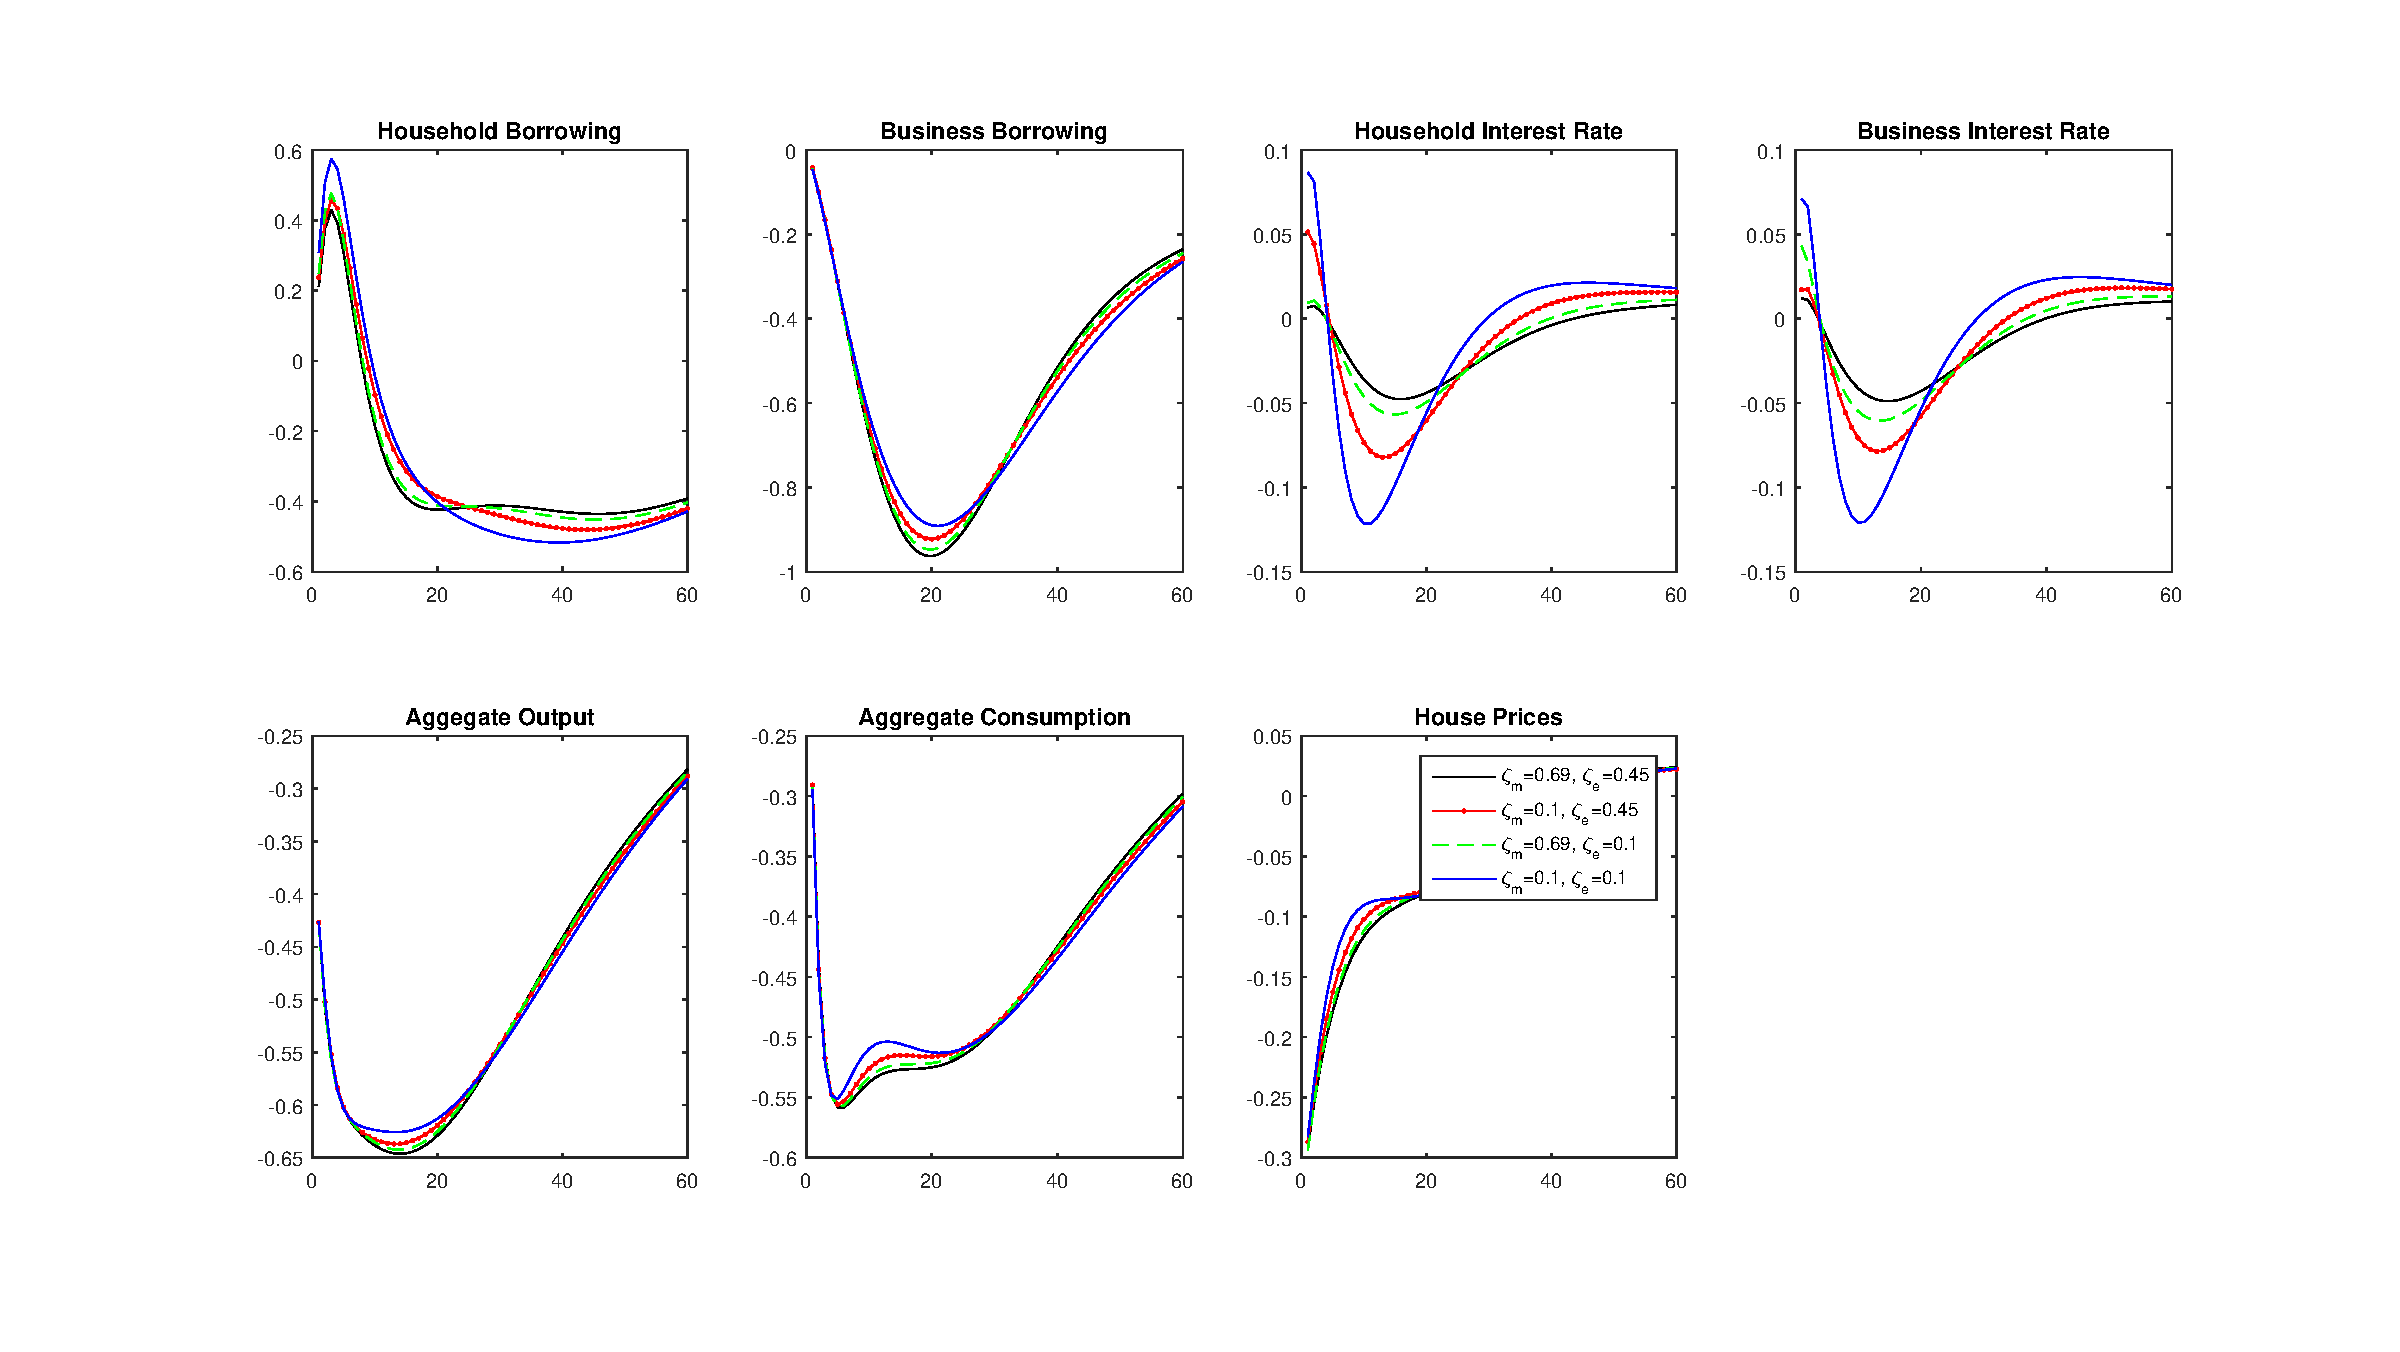
\includegraphics[scale=0.3]{stickinessA.pdf}
\end{figure}



\end{frame}



\begin{frame}{Interest-rate Stickiness on Shock Propagation-II}



\begin{figure}[H]
\centering
\caption{Bank Capital Shock}
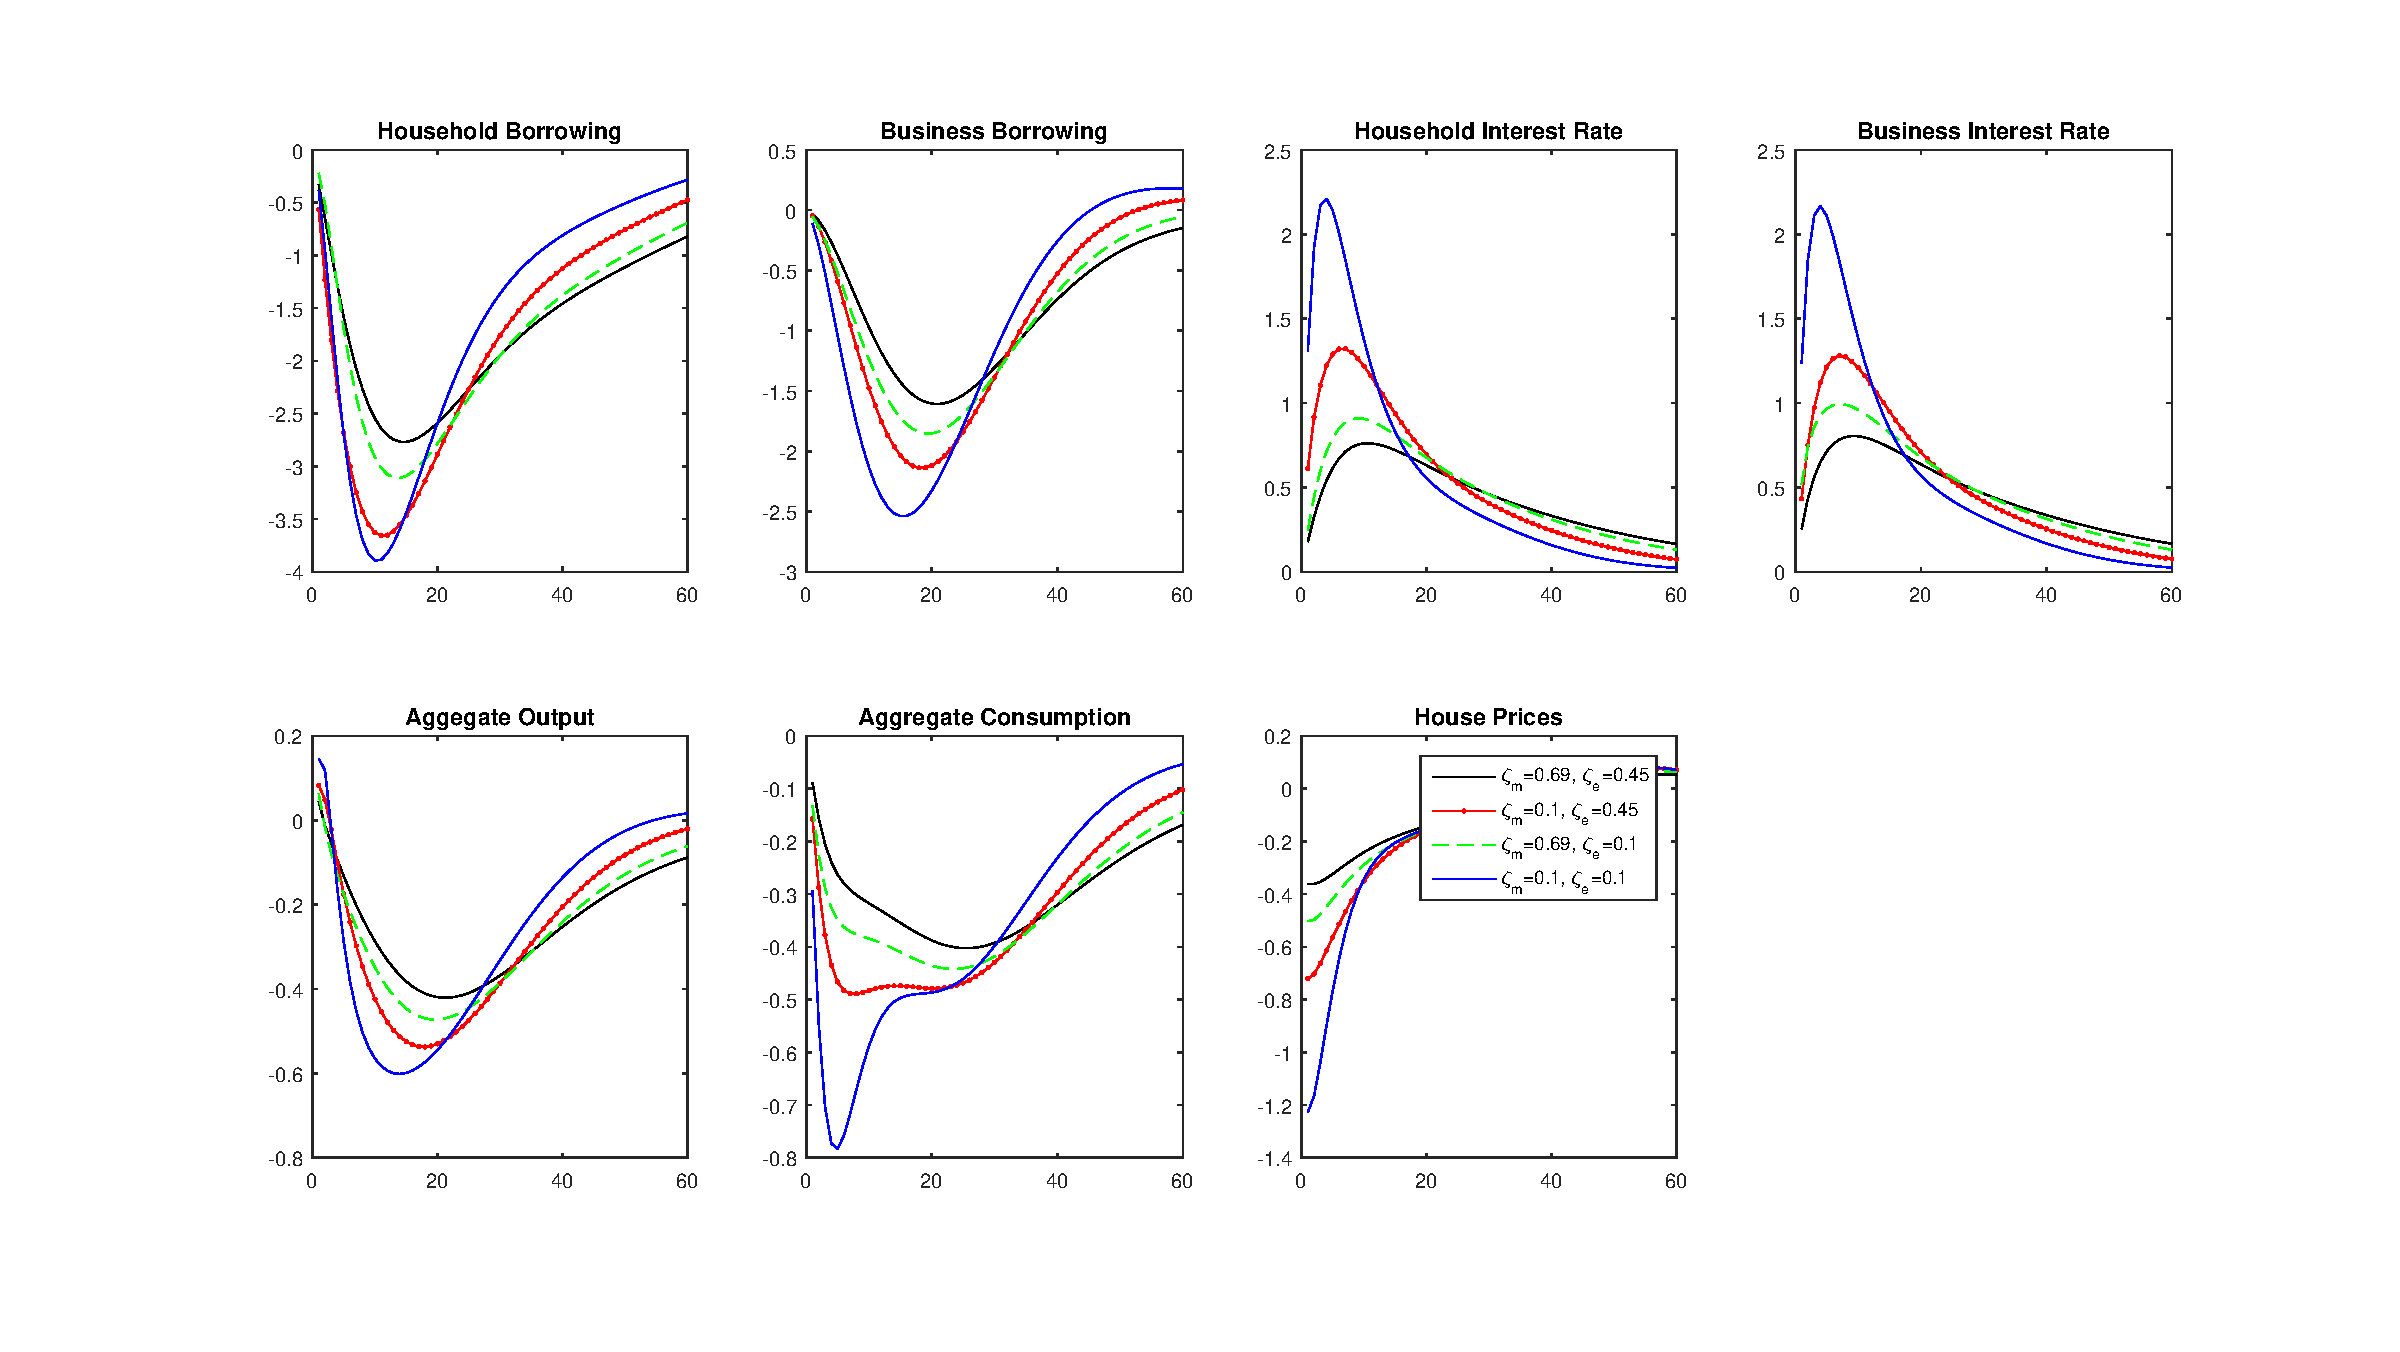
\includegraphics[scale=0.3]{stickinessCAB.pdf}
\end{figure}



\end{frame}



\begin{frame}{Interest Rate Pass-through \& Prudential Policy Interactions-I}


\begin{figure}[h]
\caption{Positive housing supply shock. Cumulative difference calculated as the  }
\subfigure[Cumulative differences: 0.24 \% and 0.59 \%.]{\includegraphics[scale=0.17]{stickiness_ccybHd.pdf}} \\
\subfigure[Cumulative differences: -2.13 \% and 0.17 \%.]{\includegraphics[scale=0.17]{stickiness_LTVHd.pdf}}
\subfigure[Cumulative differences: 0.36 \% and 0.92 \%.]{\includegraphics[scale=0.17]{stickiness_CARHd.pdf}}
\end{figure}


\end{frame}








\begin{frame}{Interest Rate Pass-through \& Prudential Policy Interactions-II}

\begin{figure}[h]
\caption{Positive bank capital shock.}
\subfigure[Cumulative differences: 2.9 \% and 2.14 \%.]{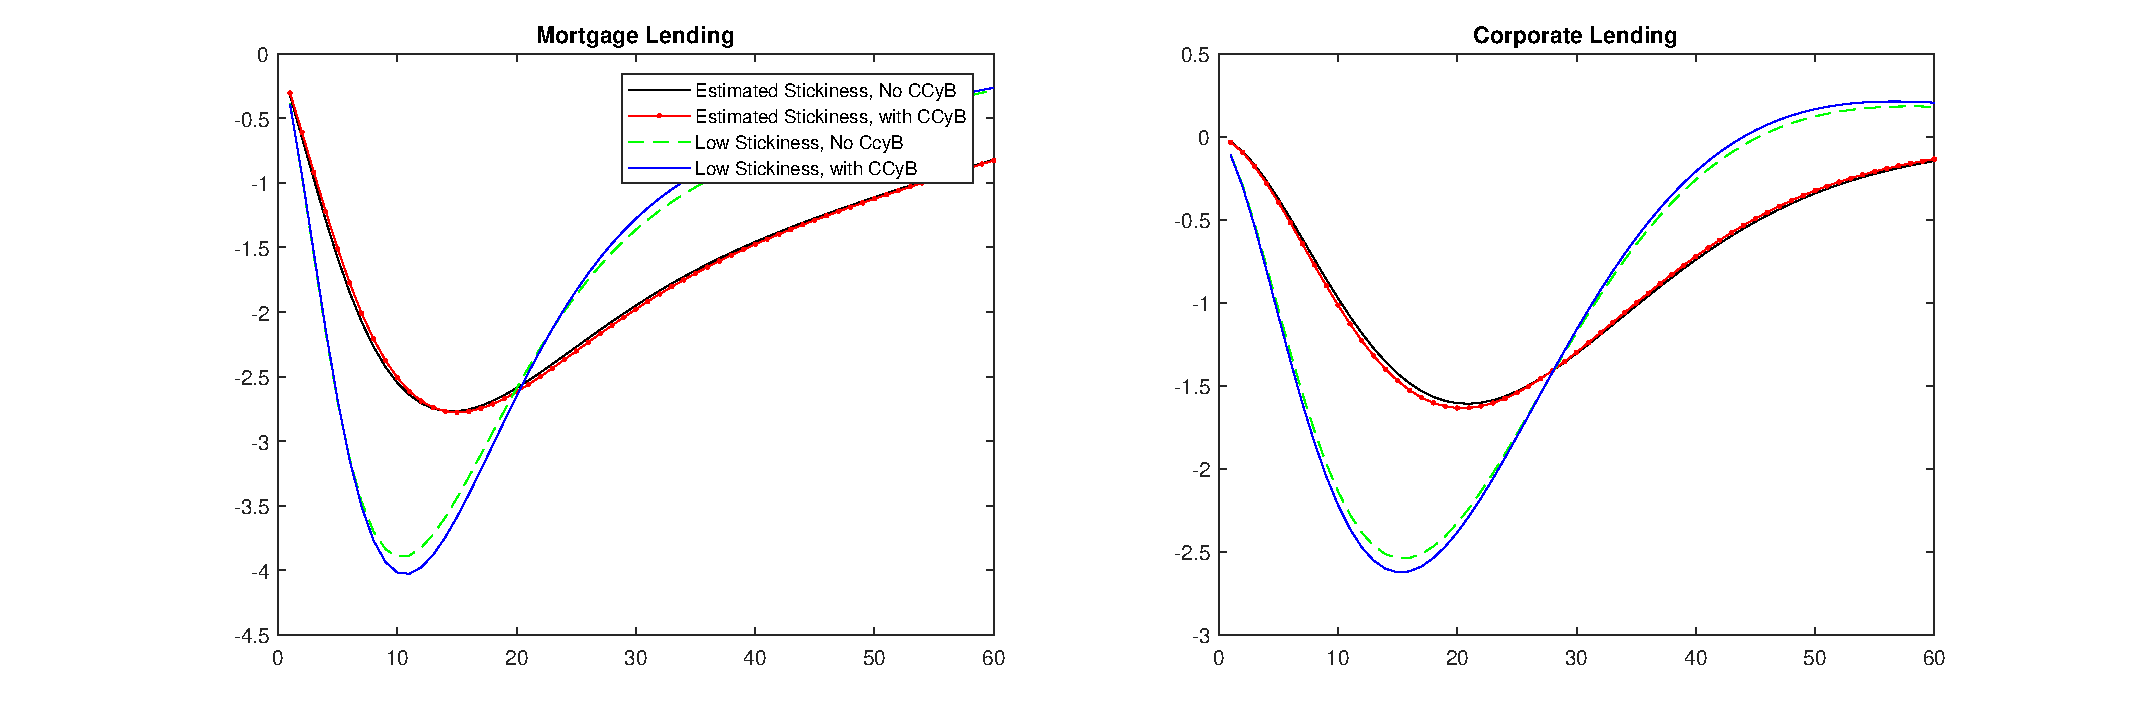
\includegraphics[scale=0.17]{stickiness_ccybECAB.pdf}}\\
\subfigure[Cumulative differences: 3.74 \% and 0.69 \%.]{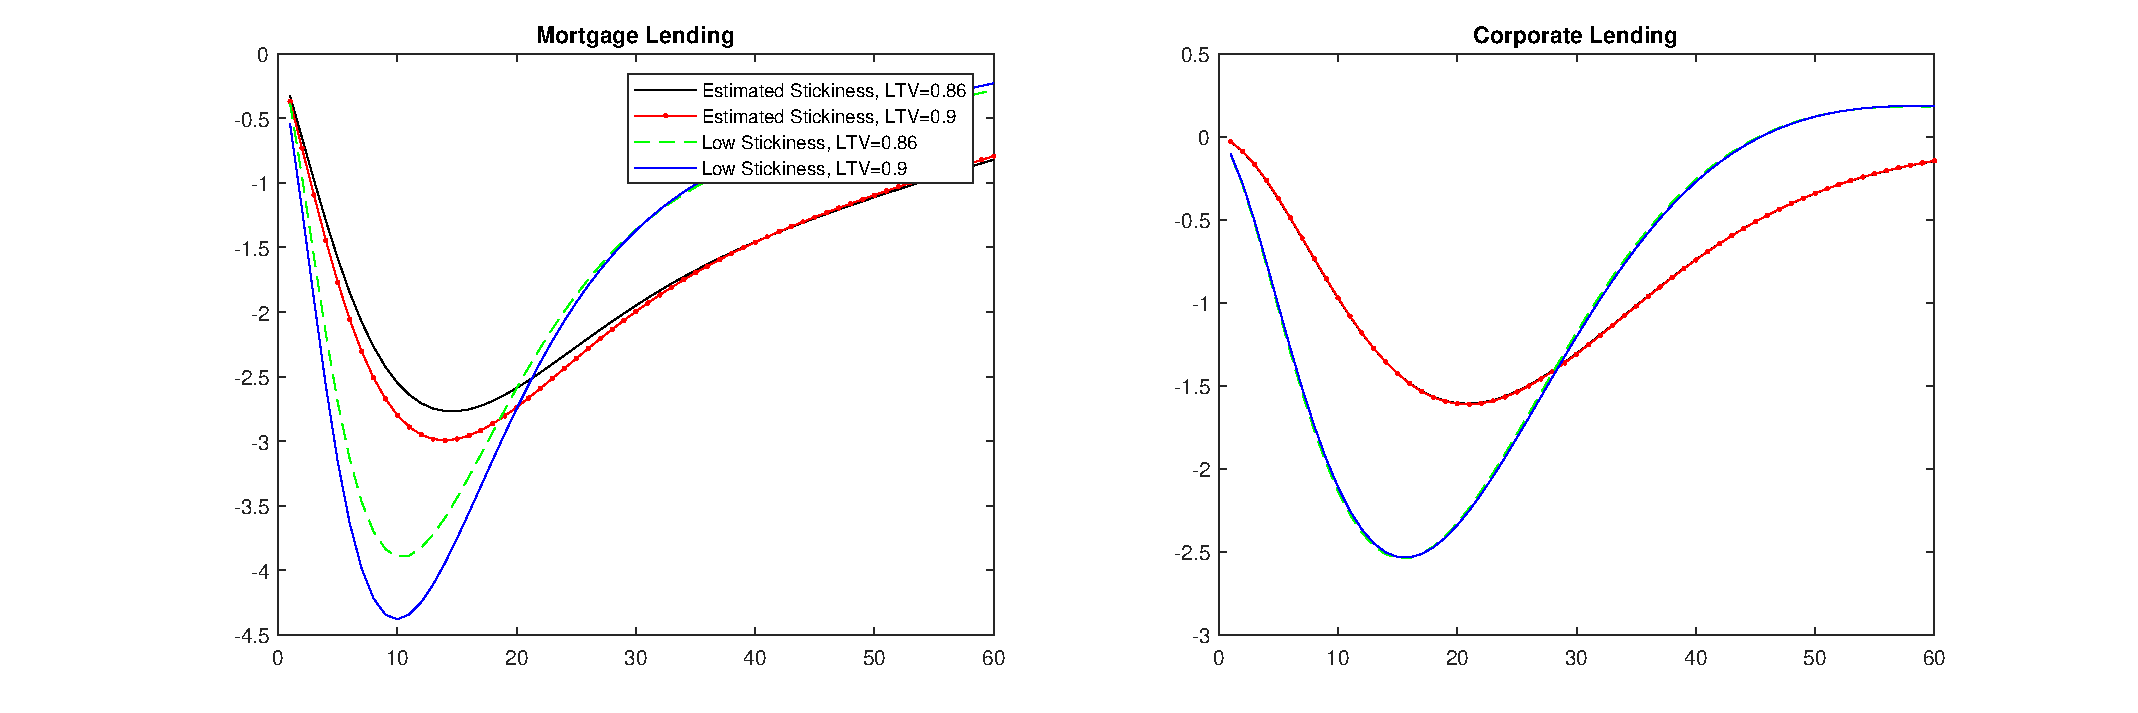
\includegraphics[scale=0.17]{stickiness_LTVECAB.pdf}}
\subfigure[Cumulative differences: 4.83 \% and 5.04 \%.]{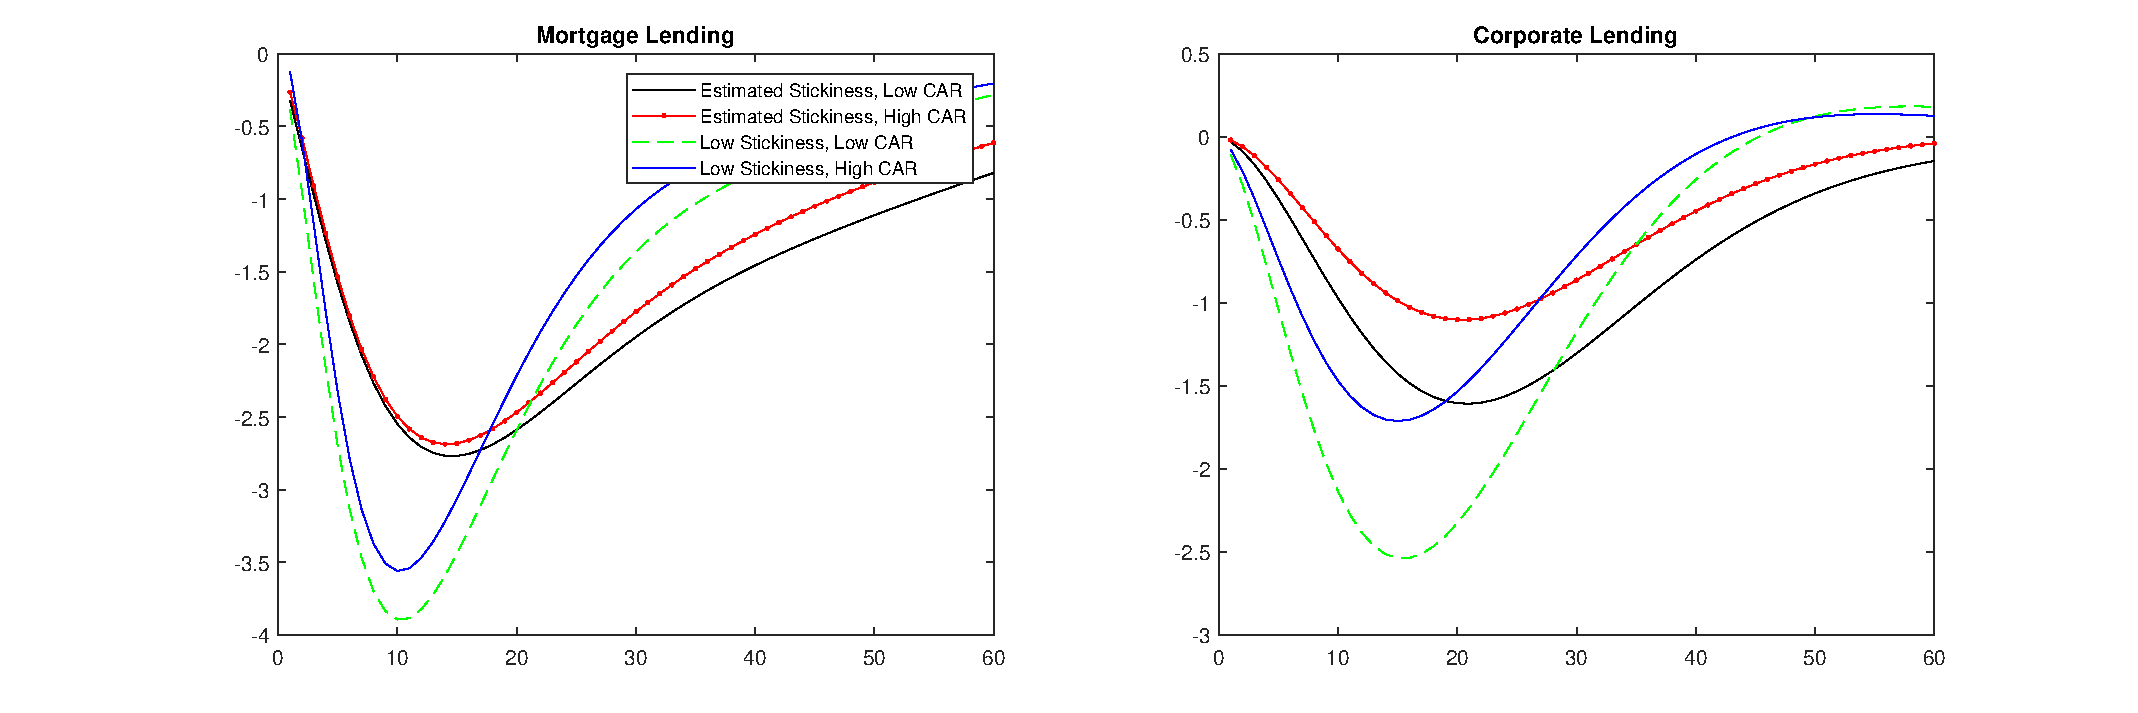
\includegraphics[scale=0.17]{stickiness_CARECAB.pdf}}
\end{figure}

\end{frame}




\end{document}

